\documentclass[11pt,oneside]{article}

\usepackage[a4paper,margin=27mm,headheight=15pt]{geometry}
\usepackage[T1]{fontenc}
\usepackage[utf8]{inputenc}
\IfFileExists{libertinus.sty}{\usepackage{libertinus}}{\usepackage{lmodern}}
\usepackage{microtype}
\usepackage{amsmath,amssymb,amsthm,mathtools,mathrsfs}
% Canonical mathematical notation for active FabiusFunction LaTeX documents.
%
% This file is intentionally a plain TeX input rather than a LaTeX package.
% Every standalone document loads it by an explicit path relative to that
% document's directory; included fragments inherit the definitions from their
% root document.  Keep this file independent of document layout and metadata.
%
% Contract:
%   * one command has one mathematical meaning throughout the active corpus;
%   * names encode semantic roles rather than a document-local choice of letter;
%   * visually similar but differently normalized objects have different print;
%   * every command below is defined normatively in the notation catalogue.
%
% The active corpus excludes docs/archive/.  Historical sources may retain
% their original notation only inside an explicitly labelled quotation.

\makeatletter
\@ifundefined{mathbb}{%
  \PackageError{fabius-notation}{The amssymb package must be loaded first}%
    {Load amsmath and amssymb before inputting fabius-notation.tex.}%
}{}
\@ifundefined{operatorname}{%
  \PackageError{fabius-notation}{The amsmath package must be loaded first}%
    {Load amsmath before inputting fabius-notation.tex.}%
}{}
\makeatother

% Version stamp used by the catalogue and by static audits.
\newcommand{\FabiusNotationVersion}{2026-08-31}

% Number systems.  NaturalNumbers is explicitly the nonnegative convention.
\newcommand{\NaturalNumbers}{\mathbb{N}_{0}}
\newcommand{\PositiveIntegers}{\mathbb{N}_{>0}}
\newcommand{\IntegerNumbers}{\mathbb{Z}}
\newcommand{\RationalNumbers}{\mathbb{Q}}
\newcommand{\RealNumbers}{\mathbb{R}}
\newcommand{\ComplexNumbers}{\mathbb{C}}
\newcommand{\ExtendedRealNumbers}{\overline{\mathbb{R}}}

% The three principal Fabius--Rvachev functions.  Subscripts are deliberate:
% a bare F and a calligraphic F have several unrelated uses in the corpus.
\newcommand{\FabiusBounded}{F_{\mathrm{bd}}}
\newcommand{\FabiusGlobal}{F_{\mathrm{gl}}}
\newcommand{\FabiusQuantile}{Q_{F}}
\newcommand{\FabiusClampedQuantile}{Q_{F,\mathrm{cl}}}
\newcommand{\RvachevUp}{\operatorname{up}}

% Constants, elementary operators, and delimiters.
\newcommand{\EulerE}{\mathrm{e}}
\newcommand{\ImaginaryUnit}{\mathrm{i}}
\newcommand{\Differential}{\mathop{}\!\mathrm{d}}
\newcommand{\AbsoluteValue}[1]{\left\lvert #1\right\rvert}
\newcommand{\Norm}[1]{\left\lVert #1\right\rVert}
\newcommand{\Floor}[1]{\left\lfloor #1\right\rfloor}
\newcommand{\Ceiling}[1]{\left\lceil #1\right\rceil}
\newcommand{\FractionalPart}[1]{\left\{#1\right\}}
\newcommand{\PositivePart}[1]{\left(#1\right)_{+}}
\newcommand{\IndicatorOf}[1]{\mathbf{1}_{#1}}
\newcommand{\SetOf}[1]{\left\{#1\right\}}
\newcommand{\InnerProduct}[1]{\left\langle #1\right\rangle}
\newcommand{\CardinalityOf}[1]{\left\lvert #1\right\rvert}
\newcommand{\DefinitionEquals}{\mathrel{\coloneqq}}
\newcommand{\Sign}{\operatorname{sgn}}
\newcommand{\IdentityOperator}{\operatorname{id}}
\newcommand{\SpanOperator}{\operatorname{span}}
\newcommand{\TraceOperator}{\operatorname{tr}}
\newcommand{\RankOperator}{\operatorname{rank}}
\newcommand{\DiagonalOperator}{\operatorname{diag}}
\newcommand{\ResidueOperator}{\operatorname*{Res}}
\newcommand{\LeastCommonMultiple}{\operatorname{lcm}}
\newcommand{\OrderOperator}{\operatorname{ord}}
\newcommand{\PrincipalLogarithm}{\operatorname{Log}}
\newcommand{\FallingFactorial}[2]{\left(#1\right)^{\underline{#2}}}
\newcommand{\RisingFactorial}[2]{\left(#1\right)^{\overline{#2}}}

% Support, topology, convolution, and metric notation.
\newcommand{\SupportOperator}{\operatorname{supp}}
\newcommand{\SupportOf}[1]{\SupportOperator\!\left(#1\right)}
\newcommand{\TopologicalSupportOf}[1]{\operatorname{tsupp}\!\left(#1\right)}
\newcommand{\Convolution}{\mathbin{*}}
\newcommand{\MetricDistance}{\operatorname{dist}}
\newcommand{\TotalVariationDistance}{d_{\mathrm{TV}}}

% Probability.  Equality and convergence in law are not metric distance.
\newcommand{\Probability}{\mathbb{P}}
\newcommand{\Expectation}{\mathbb{E}}
\newcommand{\Variance}{\operatorname{Var}}
\newcommand{\Covariance}{\operatorname{Cov}}
\newcommand{\LawOperator}{\operatorname{Law}}
\newcommand{\LawOf}[1]{\LawOperator\!\left(#1\right)}
\newcommand{\EqualInLaw}{\mathrel{\overset{\mathrm{law}}{=}}}
\newcommand{\ConvergesInLaw}{\mathrel{\xrightarrow{\mathrm{law}}}}

% Fourier and integral transforms.  The printed labels expose normalization.
% FourierTwoPi uses exp(-2*pi*i*x*xi); FourierAngular uses exp(-i*x*omega).
\newcommand{\FourierTwoPi}[1]{\widehat{#1}_{\,2\pi}}
\newcommand{\FourierAngular}[1]{\widehat{#1}_{\,\mathrm{ang}}}
\newcommand{\LaplaceTransformSymbol}{\mathcal{L}}
\newcommand{\MellinTransformSymbol}{\mathcal{M}}
\newcommand{\LaplaceTransformOf}[1]{\LaplaceTransformSymbol\!\left[#1\right]}
\newcommand{\MellinTransformOf}[1]{\MellinTransformSymbol\!\left[#1\right]}
\newcommand{\MomentGeneratingFunction}[1]{M_{#1}}
\newcommand{\CharacteristicFunction}[1]{\varphi_{#1}}

% The two standard sinc functions must never share one symbol.
\newcommand{\SincRad}{\operatorname{sinc}_{\mathrm{rad}}}
\newcommand{\SincPi}{\operatorname{sinc}_{\pi}}

% Binary arithmetic and Thue--Morse notation.
\newcommand{\BinaryDigitSum}{\operatorname{wt}_{2}}
\newcommand{\ThueMorseSignSymbol}{\varepsilon}
\newcommand{\ThueMorseSign}[1]{\varepsilon_{#1}}
\newcommand{\PadicValuation}[1]{\nu_{#1}}
\newcommand{\TwoAdicValuation}{\nu_{2}}

% q-series notation.  Every base is an explicit argument.
\newcommand{\QPochhammer}[3]{\left(#1;#2\right)_{#3}}
\newcommand{\GaussianBinomial}[3]{%
  \genfrac{[}{]}{0pt}{}{#1}{#2}_{#3}%
}
\newcommand{\QInteger}[2]{\left[#1\right]_{#2}}

% Named special functions.
\newcommand{\Polylogarithm}{\operatorname{Li}}
\newcommand{\LambertW}{W}
\newcommand{\GammaFunction}{\Gamma}
\newcommand{\RiemannZeta}{\zeta}

% Asymptotics.  BigO and LittleO are operator tokens for existing formula
% grammar; prefer the At forms so that the limiting regime is printed.
\newcommand{\BigO}{\mathcal{O}}
\newcommand{\LittleO}{o}
\newcommand{\BigOAt}[2]{\mathcal{O}_{#2}\!\left(#1\right)}
\newcommand{\LittleOAt}[2]{o_{#2}\!\left(#1\right)}

\usepackage{bm}
\usepackage{booktabs,longtable,array,tabularx}
\usepackage{graphicx}
\usepackage{pgfplots}
\usepackage{xcolor}
\usepackage{enumitem}
\usepackage{fancyhdr}
\usepackage{titlesec}
\usepackage{listings}
\usepackage{xurl}
\usepackage{hyperref}
\usepackage[nameinlink,noabbrev]{cleveref}

\definecolor{linkblue}{RGB}{25,75,135}
\definecolor{shadegray}{RGB}{246,247,249}
\definecolor{rulegray}{RGB}{195,201,208}
\pgfplotsset{compat=1.18}
\hypersetup{
  colorlinks=true,
  linkcolor=linkblue,
  citecolor=linkblue,
  urlcolor=linkblue,
  pdftitle={Nowhere Analyticity of Every Positive Compositional Iterate of the Inverse Fabius Function},
  pdfauthor={Research report prepared for the ProveIt Fabius-function corpus},
  pdfsubject={Inverse Fabius function, compositional iterates, formal power-series reversion, Rvachev up-function, and Thue--Morse sequence},
  pdfkeywords={inverse Fabius function, nowhere analytic, composition, formal reversion, Rvachev, Thue--Morse, Bell polynomials}
}

\pagestyle{fancy}
\fancyhf{}
\fancyhead[L]{\small Inverse Fabius compositional iterates}
\fancyhead[R]{\small\nouppercase{\leftmark}}
\fancyfoot[C]{\thepage}
\renewcommand{\headrulewidth}{0.4pt}

\titleformat{\section}{\Large\bfseries}{\thesection}{0.7em}{}
\titleformat{\subsection}{\large\bfseries}{\thesubsection}{0.7em}{}
\titleformat{\subsubsection}{\normalsize\bfseries}{\thesubsubsection}{0.7em}{}
\setcounter{secnumdepth}{3}
\setcounter{tocdepth}{2}
\setlist[itemize]{leftmargin=2em,itemsep=0.25em,topsep=0.4em}
\setlist[enumerate]{leftmargin=2.3em,itemsep=0.25em,topsep=0.4em}

% Long unbreakable inline mathematics occasionally leaves a line with no legal
% break point.  A small emergency stretch lets TeX loosen such a line rather
% than let it protrude into the margin; it applies only to lines that would
% otherwise be overfull.
\setlength{\emergencystretch}{2em}

\newtheorem{theorem}{Theorem}[section]
\newtheorem{proposition}[theorem]{Proposition}
\newtheorem{lemma}[theorem]{Lemma}
\newtheorem{corollary}[theorem]{Corollary}
\newtheorem{conjecture}[theorem]{Conjecture}
\theoremstyle{definition}
\newtheorem{definition}[theorem]{Definition}
\newtheorem{algorithm}[theorem]{Algorithm}
\newtheorem{example}[theorem]{Example}
\theoremstyle{remark}
\newtheorem{remark}[theorem]{Remark}
\newtheorem{warning}[theorem]{Warning}

\newcommand{\repo}{\nolinkurl{Analysis/FabiusFunction}}
\newcommand{\lean}[1]{%
  \ifmmode\text{\nolinkurl{#1}}\else\nolinkurl{#1}\fi}
\newcommand{\leanevaltwo}[1]{%
  \nolinkurl{integral_eval}\texttt{\textsubscript{2}}\nolinkurl{#1}}

\newenvironment{proofidea}{\par\smallskip\noindent\textit{Proof architecture.}\ }{\hfill$\square$\par\smallskip}
\newenvironment{boxedremark}{%
  \par\smallskip\noindent\begin{center}\begin{minipage}{0.94\textwidth}%
  \color{black}\hrule\vspace{0.6em}\small
}{%
  \vspace{0.6em}\hrule\end{minipage}\end{center}\smallskip
}

\lstdefinestyle{pseudo}{
  basicstyle=\ttfamily\small,
  backgroundcolor=\color{shadegray},
  frame=single,
  rulecolor=\color{rulegray},
  columns=fullflexible,
  keepspaces=true,
  showstringspaces=false,
  xleftmargin=0.7em,
  xrightmargin=0.7em,
  aboveskip=0.8em,
  belowskip=0.8em
}

% Report-specific notation used below.
\newcommand{\D}{\mathcal D}
\newcommand{\eps}{\varepsilon}
\newcommand{\id}{\operatorname{id}}
\newcommand{\comp}{\mathbin{\circ}}
\newcommand{\ThetaF}{\Theta}
\newcommand{\half}{\tfrac12}
\newcommand{\rad}{\operatorname{rad}}
\newcommand{\statusnote}[1]{%
  \begin{center}
  \fcolorbox{linkblue}{shadegray}{\parbox{0.91\textwidth}{\small #1}}
  \end{center}
}

\title{\textbf{Nowhere Analyticity of Every Positive\\Compositional Iterate of the Inverse Fabius Function}\\[0.5em]
\large Formal reversion, analytic inversion, and the dyadic-spine theorem}
\author{Research report prepared for the ProveIt Fabius-function corpus}
\date{30 August 2026}

\begin{document}
\maketitle

\statusnote{\textbf{Result status.}
The inverse nowhere-analytic conclusion is already a corollary of the corrected
forward-iterate report; this derived companion supplies the expanded formal-radius,
center-jet, and iterated-endpoint analysis.  A hostile repository review ported the
forward report's uniform defect estimate, corrected two-spine hypothesis, literal
$n=1$ empty tie set, and live module name.  The one-fold inverse analytic-locus and
endpoint H\"older obstructions have exact Lean counterparts.  The finite positive-list
defect arithmetic is also exhaustively formalized in \path{PartitionDefect.lean}, but
the set-partition wrapper and weighted Bell/spine estimates are not.  The forward and
inverse iterate theorems for $n\geq2$, formal-radius transport, iterated endpoint
scale, and all report conjectures remain manuscript mathematics.  The numerical
script reproduced all seven outputs byte-for-byte in a pinned environment; this
finite-order replay is not proof.  Former Conjecture 14.2 is already discharged, and
former Conjecture 14.4 duplicates the forward report.  The inverse clause of former
Conjecture 14.1 is false because formal reversion does not preserve eventual jet
vanishing.  All three appear below only as numbered quarantine warnings.}

\begin{abstract}
Let $F\colon[0,1]\to[0,1]$ be the bounded Fabius function, let
$I=F^{-1}$, and write
\[
 G_n=F^{\comp n},\qquad K_n=I^{\comp n}=G_n^{-1}.
\]
We prove that for every integer $n\geq1$, the inverse iterate $K_n$ is real analytic at
no point of $[0,1]$.  The statement is strengthened in two directions.  First, there is
a co-countable dense set $Y_n\subset(0,1)$ on which the formal Taylor series of $K_n$
has radius of convergence zero.  Second, at either endpoint $K_n$ is not even H\"older
continuous of any positive order.  At the exceptional fixed point $1/2$, by contrast,
the complete Taylor series is the affine polynomial
\[
 \frac12+2^{-n}\left(y-\frac12\right),
\]
but this polynomial does not represent $K_n$ on any neighborhood.  Thus the proof
carefully separates nowhere analyticity from divergence of the formal Taylor series.

The interior argument rests on a complete proof of the forward-iterate theorem.  The
exact derivative atlas
\[
 F^{(m)}(x)=Q_m\Theta(2^m x),\qquad Q_m=2^{\binom{m+1}{2}},
\]
is inserted into the set-partition form of Fa\`a di Bruno's formula.  A quadratic
partition defect suppresses every genuinely branched chain-rule tree, leaving a finite
sum of orbit spines.  Strictly monotone orbit slopes produce a unique dominant spine
away from a finite tie set, and binary digit transitions keep its Thue--Morse amplitude
bounded away from zero along infinitely many orders.  Hence $G_n$ has zero Taylor
radius on a co-countable dense set $E_n$.  A general convergence-invariance theorem for
formal series under smooth local inversion then gives
$Y_n=G_n(E_n)$ and the corresponding zero-radius conclusion for $K_n$.

The report also derives the iterated endpoint scale
\[
 -\log K_n(y)\sim(2\log2)^{1-2^{-n}}
       \bigl(\log(1/y)\bigr)^{2^{-n}},\qquad y\downarrow0,
\]
explains the q-binomial, sinc-product, Bell--Bernoulli, Lambert--$W$, and Legendre
connections, supplies reproducible arbitrary-precision series-reversion experiments,
and records concrete conjectures and a Lean formalization plan.
\end{abstract}

\begingroup
\small
\tableofcontents
\endgroup
\newpage

\section{Statement of the problem and strengthened results}
\label{sec:statement}

The bounded Fabius function is the unique smooth increasing bijection
$F\colon[0,1]\to[0,1]$ satisfying
\begin{equation}
 F(0)=0,\qquad F(1-x)=1-F(x),\qquad F'(x)=2F(2x)
 \quad(0\leq x\leq\half),
 \label{eq:basic-F}
\end{equation}
with the usual constant continuation outside $[0,1]$ when the bounded totalization is
used.  Put
\begin{equation}
 I:=F^{-1},\qquad G_n:=F^{\comp n},\qquad K_n:=I^{\comp n},
 \qquad G_0=K_0=\id.
 \label{eq:iterates}
\end{equation}
Associativity of composition gives the exact inverse identity
\begin{equation}
 K_n=G_n^{-1},\qquad G_n=K_n^{-1}.
 \label{eq:iterate-inverse-identity}
\end{equation}
The inverse is $C^\infty$ on $(0,1)$, though it has singular endpoint slopes.

\begin{theorem}[Main theorem: inverse iterates are nowhere analytic]
\label{thm:inverse-main}
For every integer $n\geq1$, the $n$-fold inverse iterate
\[
 K_n=I^{\comp n}
\]
is not real analytic at any point of $[0,1]$.
\end{theorem}

The proof yields a stronger statement about formal Taylor series.  For a smooth
function $h$ near $x$, write
\[
 R_h(x):=\rad\sum_{m\geq0}\frac{h^{(m)}(x)}{m!}z^m
\]
for the radius of convergence of its formal Taylor series; the series need not
represent $h$ even when this radius is positive.

\begin{theorem}[Co-countable zero-radius set for inverse iterates]
\label{thm:inverse-strong}
For each fixed $n\geq1$ there exists a co-countable dense set
$Y_n\subset(0,1)$ such that
\begin{equation}
 R_{K_n}(y)=0,
 \qquad
 \limsup_{m\to\infty}
 \left(\frac{|K_n^{(m)}(y)|}{m!}\right)^{1/m}=+\infty
 \quad(y\in Y_n).
 \label{eq:inverse-zero-radius}
\end{equation}
More precisely, one may take $Y_n=G_n(E_n)$, where the explicit co-countable dense set
$E_n$ is defined in \eqref{eq:En} from forward orbit arithmetic.
\end{theorem}

The exceptional points are genuine and instructive.

\begin{theorem}[Affine but nonrepresenting center jet]
\label{thm:center-jet}
For every $n\geq1$,
\begin{equation}
 K_n(\half)=\half,\qquad K_n'(\half)=2^{-n},\qquad
 K_n^{(m)}(\half)=0\quad(m\geq2).
 \label{eq:center-jet}
\end{equation}
Thus the Taylor series of $K_n$ at $1/2$ is an affine polynomial of infinite radius,
but it does not agree with $K_n$ on any neighborhood.
\end{theorem}

The forward theorem needed for the proof is itself stronger than nowhere analyticity.

\begin{theorem}[Forward engine theorem]
\label{thm:main}
For every integer $n\geq1$, $G_n=F^{\comp n}$ is not real analytic at any point of
$[0,1]$.
\end{theorem}

\begin{theorem}[Forward co-countable zero-radius set]
\label{thm:strong}
Fix $n\geq1$.  There exists a co-countable dense set $E_n\subset(0,1)$ such that, for
every $x\in E_n$,
\begin{equation}
 \limsup_{m\to\infty}
 \left(\frac{|G_n^{(m)}(x)|}{m!}\right)^{1/m}=+\infty.
 \label{eq:infinite-limsup}
\end{equation}
Consequently $R_{G_n}(x)=0$ for every $x\in E_n$.
\end{theorem}

The logical order of the report is deliberate.  We first establish the forward engine
by a derivative-spine argument.  We then transfer both nonanalyticity and zero Taylor
radius through local inversion.  The endpoint and center analyses are treated
separately because the inverse is not a local diffeomorphism at the endpoints and
because the center has a convergent but nonrepresenting Taylor series.

\section{Repository audit and novelty boundary}
\label{sec:audit}

The source audit was organized around the repository's canonical documents and its
own consolidation manifests.  This is important because the tree contains live
proof-backed expositions, a formal Lean development, canonical frontier syntheses,
and many frozen or mechanically merged historical drafts.  Treating every duplicate
as an independent source would obscure rather than improve provenance.

\subsection{Canonical sources inspected}

The following live documents form the mathematical backbone of the present report.
\begin{longtable}{@{}p{0.30\textwidth}p{0.62\textwidth}@{}}
\toprule
Repository document & Role in the present proof \\
\midrule
\endhead
\texttt{Fabius\_Function\_and\_}\newline\texttt{Rvachev\_Up.tex}
& Primary proof-backed exposition: definitions, symmetry, strict monotonicity,
convexity and concavity, the signed global extension, exact all-order derivative
formulae, sharp derivative bounds, dyadic jets, inverse-function facts, and the
formal base nowhere-analyticity statement.\\[0.4em]
\texttt{Fabius\_Function\_}\newline\texttt{Mathematical\_}\newline\texttt{Glossary.tex}
& Notation and cross-reference audit, including the bounded function, signed global
extension, Rvachev bump, dyadic grids, Thue--Morse signs, and analytic-locus language.\\[0.4em]
\texttt{Non\_Elementarity\_}\newline\texttt{of\_the\_Fabius\_}\newline\texttt{Function.tex}
& Dense analyticity of elementary-function classes, the exact analytic locus of $F$,
and the corresponding obstruction for $F^{-1}$.\\[0.4em]
\texttt{fabius\_lean\_}\newline\texttt{walkthrough.tex}
& Module-level proof map for the formal derivative, flatness, inverse, and
nowhere-analyticity results.\\[0.4em]
\texttt{semi-formalized-}\newline\texttt{research-frontiers.tex}
& Canonical synthesis of q-binomial, sinc-product, Lambert--$W$, Bell/Bernoulli,
Legendre, inverse, sampling, and asymptotic directions.\\[0.4em]
\bottomrule
\end{longtable}

The archive index and the semi-formalized-frontier README were used as provenance
crosswalks for first versions, absorbed notebooks, mechanically merged draft groups,
and editorial syntheses.  Thus historical copies were audited through their canonical
successors and checksummed consolidation records rather than cited as competing
statements.  The repository itself explicitly separates proof-backed claims from
frontier statements awaiting literal formal counterparts; this report follows the
same convention.

\subsection{Existing results and the novelty boundary}

The repository already proves the exact analytic locus of the bounded function,
\begin{equation}
 F\text{ is analytic at }x\quad\Longleftrightarrow\quad x\notin[0,1],
 \label{eq:base-locus}
\end{equation}
and proves the corresponding one-fold statement for $I=F^{-1}$.  The inverse proof
uses positivity of $F'$ on $(0,1)$, the real-analytic inverse-function theorem, and a
separate endpoint obstruction.  These results settle $n=1$ but do not by themselves
settle $n\geq2$.

There are two nontrivial gaps to bridge.  First, nowhere analyticity is not preserved by
composition for arbitrary smooth functions: chain-rule cancellation may remove a
singularity, and eventual vanishing of one jet does not imply eventual vanishing after
composition.  Second, even after proving the forward theorem for $G_n$, one still needs
to distinguish three inverse questions: local analytic representability, convergence
of the formal inverse Taylor series, and endpoint regularity.  The present report
addresses all three.

The corrected sibling report
\path{drafts/representations/fabius_iterates_nowhere_analytic/} now proves the all-$n$
forward theorem and already records inverse nowhere analyticity as a corollary.
Accordingly, Sections \ref{sec:defect}--\ref{sec:proof-main} are a derived copy of that
forward engine, not independent novelty.  They are retained here so the inverse
argument can be read in one document, with all corrections from the sibling report
ported verbatim.  The distinct manuscript layer begins in
Section \ref{sec:inverse-transfer}: formal Taylor-radius transport through smooth local
inversion, the affine but nonrepresenting center jet, and the iterated inverse endpoint
scale.  The corpus formalizes the $n=1$ inverse analytic locus and one-fold endpoint
H\"older obstruction, but it does not yet contain exact Lean counterparts for these
$n\geq2$ iterate statements.

\section{Fabius, Rvachev, Thue--Morse, and the derivative atlas}
\label{sec:background}

\subsection{The Rvachev bump and the signed global extension}

Let $\RvachevUp$ denote Rvachev's compactly supported $C^\infty$ function, normalized by
\[
 \SupportOperator\RvachevUp=[-1,1],\qquad \RvachevUp(0)=1,
\]
and related to the bounded Fabius function by
\begin{equation}
 \RvachevUp(t)=F(1-\AbsoluteValue t)\qquad(-1\leq t\leq1).
 \label{eq:up-F}
\end{equation}
In particular, $\RvachevUp$ is even, strictly decreasing on $[0,1]$, and
\begin{equation}
 \RvachevUp(\half)=F(\half)=\half.
 \label{eq:up-half}
\end{equation}

For $k\geq0$, put
\begin{equation}
  \eps_k=(-1)^{s_2(k)},
  \label{eq:tm-sign}
\end{equation}
where $s_2(k)$ is the sum of the binary digits of $k$.  The signed global extension
$\ThetaF$ can be written blockwise as
\begin{equation}
 \ThetaF(t)=\eps_k\,\RvachevUp\bigl(t-(2k+1)\bigr),
 \qquad 2k\leq t\leq2k+2.
 \label{eq:theta-block}
\end{equation}
It agrees with $F$ on $[0,1]$, satisfies $\ThetaF'(t)=2\ThetaF(2t)$ globally, and obeys
\begin{equation}
 \AbsoluteValue{\ThetaF(t)}\leq1.
 \label{eq:theta-bound}
\end{equation}
The translate signs in \eqref{eq:theta-block} are precisely the Thue--Morse signs.

\subsection{Exact all-order derivatives}

Define the superfactorial dyadic scale
\begin{equation}
  Q_m:=2^{\binom{m+1}{2}}=2^{m(m+1)/2}.
  \label{eq:Qm}
\end{equation}
Repeated differentiation of the dilation equation gives, for every $m\geq1$ and
$x\in(0,1)$,
\begin{equation}
  F^{(m)}(x)=Q_m\ThetaF(2^m x).
  \label{eq:derivative-atlas}
\end{equation}
Consequently
\begin{equation}
  \AbsoluteValue{F^{(m)}(x)}\leq Q_m.
  \label{eq:F-derivative-bound}
\end{equation}
At the matched dyadic grid this becomes the exact Thue--Morse jet law
\begin{equation}
 F^{(m)}\!\left(\frac{a}{2^m}\right)
 =\begin{cases}
 0,&a\text{ even},\\
 Q_m\eps_{\lfloor a/2\rfloor},&a\text{ odd}.
 \end{cases}
 \label{eq:dyadic-jet}
\end{equation}
The factor $Q_m$ is the source of nonanalytic growth.  Since
\begin{equation}
  Q_m^{1/m}=2^{(m+1)/2},
  \label{eq:Q-root}
\end{equation}
no fixed ordinary exponential can neutralize it after division by $m!$.
The only serious issue is cancellation among the many chain-rule terms created by
composition.

\subsection{Shape and orbit dynamics}

The repository proves that $F$ is a strictly increasing bijection of $[0,1]$, that
$F'$ is strictly increasing on $[0,\half]$ and strictly decreasing on
$[\half,1]$, and that
\begin{equation}
 F'(0)=0,\qquad F'(\half)=2,\qquad F'(1)=0.
 \label{eq:slope-values}
\end{equation}
Moreover $F$ is strictly convex on $[0,\half]$ and strictly concave on
$[\half,1]$.  Comparing with the chord joining $(0,0)$ and $(\half,\half)$ gives
\begin{equation}
  F(x)<x\quad(0<x<\half),
  \qquad
  F(x)>x\quad(\half<x<1).
  \label{eq:drift}
\end{equation}
Thus every noncentral interior orbit moves monotonically toward an endpoint:
\begin{align}
 0<x<\half&\implies x>F(x)>F^{\comp2}(x)>\cdots>0,
 \label{eq:left-orbit}\\
 \half<x<1&\implies x<F(x)<F^{\comp2}(x)<\cdots<1.
 \label{eq:right-orbit}
\end{align}
This elementary dynamical fact will force strict unimodality of the exponential
weights in the derivative spine sum.

\section{Why a direct dyadic-jet induction fails}

It is useful to see the obstruction before introducing the cure.  For two smooth
functions $f$ and $h$,
\begin{equation}
 (f\comp h)^{(m)}(x)
 =\sum_{\pi\in\Pi_m}
 f^{(|\pi|)}(h(x))\prod_{B\in\pi}h^{(|B|)}(x),
 \label{eq:faa-set-partitions}
\end{equation}
where $\Pi_m$ is the set of partitions of $\SetOf{1,\ldots,m}$.  Even if
$h^{(r)}(x)=0$ for all large $r$, partitions with many small blocks can survive.
Similarly, even if the high derivatives of $f$ vanish at $h(x)$, the term
$f'(h(x))h^{(m)}(x)$ survives.  There is no pointwise ``eventually zero jet''
induction for $F^{\comp n}$.

At the opposite extreme, a crude absolute-value bound on \eqref{eq:faa-set-partitions}
introduces Bell numbers.  Since the number of partitions is superexponential on an
ordinary exponential scale, such a bound loses the delicate comparison with $Q_m$.
The correct normalization must exploit the quadratic exponent in $Q_m$, not merely
count partitions.  This leads to the defect below.

\section{The dyadic defect of a Fa\`a di Bruno partition}
\label{sec:defect}

Let $\pi\in\Pi_m$ have $k=|\pi|$ blocks of sizes
$r_1,\ldots,r_k$, so $r_1+\cdots+r_k=m$.  Define
\begin{equation}
 D(\pi):=\binom m2-\binom k2-\sum_{i=1}^k\binom{r_i}{2}.
 \label{eq:defect}
\end{equation}
An equivalent and more transparent formula is
\begin{equation}
 D(\pi)=\sum_{1\leq i<j\leq k}(r_ir_j-1).
 \label{eq:defect-pairs}
\end{equation}
Every summand is nonnegative.  Therefore $D(\pi)=0$ only in the two extremal cases:
there is one block, or every block is a singleton.  These are exactly the two
unbranched chain-rule spines.

\paragraph{Lean crosswalk: the finite positive-list defect is complete.}
\begingroup\small\sloppy
The module \path{PartitionDefect.lean} has exactly three public definitions
and thirty-three public theorems; the following inventory is exhaustive.
Its list \(r=[r_1,\ldots,r_k]\) records positive block sizes, but it does not
construct a set partition of \(\{1,\ldots,m\}\).
\begin{itemize}[leftmargin=2em]
 \item The three definitions are \path{pairSum}, \path{blockPairDefect}, and
 \path{partitionDefect}.
 \item The unordered-pair and triangular-number engine consists of
 \path{pairSum_nil}, \path{pairSum_cons}, \path{pairSum_one},
 \path{pairSum_add}, \path{pairSum_congr}, \path{pairSum_map},
 \path{choose_add_two}, and \path{choose_list_sum_two}.
 \item The conventional defect formulas, excess decomposition, and fixed-block
 lower bound are
 \path{blockPairDefect_eq_mul_sub_one},
 \path{partitionDefect_eq_pairSum_mul_sub_one},
 \path{partitionDefect_nonneg},
 \path{choose_sum_two_eq_choose_length_add_sum_add_partitionDefect},
 \path{partitionDefect_eq_choose_sum_sub_choose_length_sub_sum},
 \path{length_le_sum_of_pos}, \path{sum_map_sub_one},
 \path{pairSum_add_eq}, \path{pairSum_map_add_eq},
 \path{partitionDefect_eq_linear_add_pairwise_excess},
 \path{partitionDefect_lower_bound}, and
 \path{partitionDefect_fixed_block_bound}.
 \item The zero and sharp-equality classifiers are
 \path{pairSum_eq_zero_iff_pairwise},
 \path{blockPairDefect_eq_zero_iff},
 \path{partitionDefect_eq_zero_iff},
 \path{sub_one_mul_sub_one_eq_zero_iff},
 \path{partitionDefect_eq_lower_bound_iff}, and
 \path{partitionDefect_fixed_block_eq_iff}.
 \item The first-positive-shell closure is
 \path{add_sub_one_le_mul_of_pos},
 \path{mul_eq_add_sub_one_iff},
 \path{firstShell_le_fixedBlockProduct},
 \path{fixedBlockProduct_eq_firstShell_iff},
 \path{firstShell_le_partitionDefect},
 \path{partitionDefect_eq_firstShell_iff}, and
 \path{partitionDefect_twoBlock_firstShell}.
\end{itemize}
For positive entries the module proves
\[
 D(r)=(k-1)\sum_i(r_i-1)
      +\sum_{i<j}(r_i-1)(r_j-1)
 \ge (k-1)(m-k).
\]
It proves \(D(r)=0\) exactly when \(k\le1\) or every entry is one; equality
in the fixed-\(m\), fixed-\(k\) bound exactly when every pair contains a
singleton (equivalently at most one entry exceeds one); and, under precisely
\(2\le k<m\), the first-shell bound \(D(r)\ge m-2\), with equality exactly at
\(k=2\) or \(k=m-1\) together with that same one-nonsingleton condition.  The
explicit profile \([m-1,1]\) attains the shell for \(m\ge3\).

This closure does \emph{not} formalize the set-partition family \(\Pi_m\),
the quadratic-scale factorization \eqref{eq:Q-factorization}, the weighted
Bell sum \eqref{eq:defect-decay}, its asymptotics, the two-spine reduction,
the finite spine expansion, or either the forward- or inverse-iterate theorem.
Those steps remain paper-only.
\endgroup

Let $u(\pi)$ be the number of singleton blocks and let
\begin{equation}
 s(\pi):=k-u(\pi)
 \label{eq:s-nonsingleton}
\end{equation}
be the number of non-singleton blocks.

\begin{lemma}[Quadratic-scale factorization]
\label{lem:Q-factorization}
For every partition $\pi\in\Pi_m$,
\begin{equation}
 \frac{Q_k\prod_{r_i\geq2}Q_{r_i}}{Q_m}
 =2^{s(\pi)-D(\pi)}.
 \label{eq:Q-factorization}
\end{equation}
\end{lemma}

\begin{proof}
Using $\log_2Q_r=r(r+1)/2$ and omitting singleton blocks from the product,
\begin{align*}
 2\log_2\frac{Q_k\prod_{r_i\ge2}Q_{r_i}}{Q_m}
 &=k(k+1)+\sum_{r_i\ge2}r_i(r_i+1)-m(m+1)\\
 &=k^2+s(\pi)+\sum_{r_i\ge2}r_i^2-m^2.
\end{align*}
On the other hand, expanding \eqref{eq:defect} gives
\[
 2D(\pi)=m^2-k^2+s(\pi)-\sum_{r_i\ge2}r_i^2.
\]
Subtracting proves \eqref{eq:Q-factorization}.
\end{proof}

The next proposition is the combinatorial engine.  Its role is stronger than saying
that each nonextremal partition has positive defect: it shows that the sum over all
of them is still exponentially small.

\begin{proposition}[Weighted defect decay]
\label{prop:defect-decay}
For each fixed $K>0$ there exist constants $C_K>0$ and $\rho_K\in(0,1)$ such that
\begin{equation}
 \sum_{\substack{\pi\in\Pi_m\\1<|\pi|<m}}
   (2K)^{s(\pi)}2^{-D(\pi)}
 \leq C_K\rho_K^m
 \qquad(m\geq2).
 \label{eq:defect-decay}
\end{equation}
\end{proposition}

\begin{proof}
We give the full counting argument because this is the point at which a naive Bell
number estimate fails.

Write $k=|\pi|$, let
\begin{equation}
 e:=m-k
 \label{eq:excess}
\end{equation}
be the total block excess over singletons, and let $r_{\max}=m-t$ be the largest block
size.  Convexity of $r\mapsto\binom r2$ shows that, for fixed $m$ and $k$, the defect
is minimized by one block of size $m-k+1$ and $k-1$ singleton blocks.  Hence
\begin{equation}
 D(\pi)\geq e(k-1)=e(m-e-1).
 \label{eq:defect-e}
\end{equation}
The contribution between a largest block and all other blocks gives the second bound
\begin{equation}
 D(\pi)\geq (m-t)t-(k-1)\geq t(m-t-1).
 \label{eq:defect-t}
\end{equation}

First consider partitions with $1\leq e\leq m/4$.  Their non-singleton blocks contain
at most $2e$ elements, because the number of such blocks is at most $e$.  Choosing
those elements and partitioning them gives at most
\begin{equation}
  (2e+1)m^{2e}(2e)^{2e}
 \label{eq:count-near-singletons}
\end{equation}
possibilities.  Also $s(\pi)\leq e$, while \eqref{eq:defect-e} gives
$D(\pi)\geq e(3m/4-1)$.  Uniformly for $1\leq e\leq m/4$, the base-two logarithm
of the counting and weight factor is at most
\[
 \log_2(2e+1)+4e\log_2m+e\log_2\max(1,2K).
\]
For fixed $K$ this is at most $em/4$ once $m$ is large enough, whereas the
negative defect exponent is at most $-e(3m/4-1)$.  Thus the $e$-th contribution
is at most $2^{-em/3}$ after enlarging the threshold once more, uniformly in
$e$.  The resulting geometric sum is $\BigO(2^{-m/3})$.

Next consider partitions with $1\leq t\leq m/4$.  Choose the $t$ elements outside a
largest block and partition them.  Up to harmless overcounting there are at most
$m^t t^t$ choices, and $s(\pi)\leq t+1$.  By \eqref{eq:defect-t},
$D(\pi)\geq t(3m/4-1)$.  The same explicit estimate as above, now with $t$ in
place of $e$ (and one harmless extra factor $\max(1,2K)$), bounds the $t$-th
contribution by $2^{-tm/3}$ for all sufficiently large $m$, uniformly for
$1\leq t\leq m/4$.  Its sum is again exponentially small.

It remains to treat the middle region $e>m/4$ and $t>m/4$.  If $t\leq3m/4$, then
\eqref{eq:defect-t} gives $D(\pi)\geq c_1m^2$ for all sufficiently large $m$ and an
absolute $c_1>0$.  Suppose instead that $t>3m/4$, so every block has size less than
$m/4$.  If $k>m/4$, then \eqref{eq:defect-e} gives
$D(\pi)\geq c_2m^2$.  If $k\leq m/4$, then
\begin{align*}
 D(\pi)
 &=\sum_{i<j}r_ir_j-\binom k2\\
 &=\frac{m^2-\sum_i r_i^2}{2}-\binom k2
 >\frac{3m^2}{8}-\frac{m^2}{32}
 =\frac{11m^2}{32}.
\end{align*}
In the middle region, the total number of partitions is at most $m^m$ and the weight
$(2K)^{s(\pi)}$ is at most $\max(1,2K)^m$.  Both are overwhelmed by
$2^{-c m^2}$.  Combining the three regions proves \eqref{eq:defect-decay}, after
increasing $C_K$ to cover the finitely many small values of $m$.
\end{proof}

\section{A two-spine composition lemma}
\label{sec:two-spine}

The weighted defect estimate converts Fa\`a di Bruno's formula into an asymptotically
binary chain rule.

\begin{lemma}[Two-spine reduction]
\label{lem:two-spine}
Let $h$ be smooth near $x$, let $f$ be smooth near $y=h(x)$, and put
$B=\AbsoluteValue{h'(x)}$.  Suppose
there are constants $H>0$ and $K\geq1$ such that
\begin{align}
 \AbsoluteValue{f^{(r)}(y)}&\leq Q_r &&(r\geq1),
 \label{eq:f-envelope}\\
 \AbsoluteValue{h^{(r)}(x)}&\leq KQ_rH^r &&(r\geq2).
 \label{eq:h-envelope}
\end{align}
Then, with $L=\max(B,H)$,
\begin{equation}
 (f\comp h)^{(m)}(x)
 =f'(y)h^{(m)}(x)+f^{(m)}(y)h'(x)^m
  +\LittleO(Q_mL^m)
 \quad(m\to\infty).
 \label{eq:two-spine}
\end{equation}
\end{lemma}

\begin{proof}
In \eqref{eq:faa-set-partitions}, remove the one-block partition and the all-singleton
partition.  They give exactly the two displayed terms.  For any remaining partition
$\pi$ with $k$ blocks, $u$ singleton blocks, and $s=k-u$ non-singleton blocks, the
corresponding term has absolute value at most
\[
 Q_k B^u\prod_{r_i\ge2}(KQ_{r_i}H^{r_i})
 \leq Q_mL^m(2K)^s2^{-D(\pi)},
\]
where \cref{lem:Q-factorization} was used in the last step.  Summing and applying
\cref{prop:defect-decay} bounds the entire remainder by
$C_KQ_mL^m\rho_K^m=\LittleO(Q_mL^m)$.
\end{proof}

\begin{remark}[Why this lemma is composition-stable]
The estimate does not require analyticity, Gevrey bounds of factorial type, or a
closed formula for every Bell polynomial.  It uses only the exact quadratic dyadic
scale $Q_r$ and an ordinary exponential envelope $H^r$ for the inner derivatives.
The conclusion has the same form, so it can be iterated a fixed number of times.
\end{remark}

\section[The orbit-spine asymptotic for compositional iterates]{The orbit-spine asymptotic for $F^{\comp n}$}
\label{sec:spines}

Fix $x\in(0,1)$ and $n\geq1$.  Define the finite orbit
\begin{equation}
  x_j:=G_j(x)=F^{\comp j}(x),\qquad 0\leq j\leq n-1,
  \label{eq:orbit}
\end{equation}
and the local slopes
\begin{equation}
  a_j:=F'(x_j)>0.
  \label{eq:slopes}
\end{equation}
The prefix and suffix weights are
\begin{align}
 B_0&:=1,
 &B_j&:=\prod_{r=0}^{j-1}a_r=G_j'(x)\quad(j\geq1),
 \label{eq:prefix}\\
 A_{j,n}&:=\prod_{r=j+1}^{n-1}a_r,
 &&0\leq j<n,
 \label{eq:suffix}
\end{align}
where empty products equal $1$.  Finally set
\begin{equation}
 H_n(x):=\max_{0\leq j<n}B_j.
 \label{eq:Hn}
\end{equation}

\begin{theorem}[Finite spine expansion]
\label{thm:spine-expansion}
For each fixed $n\geq1$ and $x\in(0,1)$,
\begin{equation}
 G_n^{(m)}(x)
 =Q_m\left[
   \sum_{j=0}^{n-1}A_{j,n}B_j^m\ThetaF(2^m x_j)
   +\LittleO\bigl(H_n(x)^m\bigr)
 \right]
 \qquad(m\to\infty).
 \label{eq:spine-expansion}
\end{equation}
\end{theorem}

\begin{proof}
We induct on $n$.  For $n=1$, $x_0=x$, $A_{0,1}=B_0=H_1=1$, and
\eqref{eq:spine-expansion} is exactly \eqref{eq:derivative-atlas}.

Assume the formula for $G_j$.  It immediately supplies a global-in-order envelope at
the fixed point $x$: there is $K\geq1$ such that
\begin{equation}
 \AbsoluteValue{G_j^{(r)}(x)}\leq KQ_rH_j(x)^r\qquad(r\geq2).
 \label{eq:Gj-envelope}
\end{equation}
Indeed the asymptotic gives the estimate for all sufficiently large $r$, and $K$ can
be enlarged to absorb the finitely many remaining orders.

Apply \cref{lem:two-spine} with $f=F$ and $h=G_j$.  Since
$h(x)=x_j$, $h'(x)=B_j$, $f'(x_j)=a_j$, and
$f^{(m)}(x_j)=Q_m\ThetaF(2^m x_j)$, we obtain
\begin{equation}
 G_{j+1}^{(m)}(x)
 =a_jG_j^{(m)}(x)
  +Q_mB_j^m\ThetaF(2^m x_j)
  +\LittleO\bigl(Q_mH_{j+1}(x)^m\bigr),
 \label{eq:spine-induction-step}
\end{equation}
where $H_{j+1}=\max(H_j,B_j)$.  Multiplication by $a_j$ changes every old suffix
factor $A_{i,j}$ into $A_{i,j+1}$, while the new term has suffix factor
$A_{j,j+1}=1$.  This is precisely \eqref{eq:spine-expansion} for $j+1$.
\end{proof}

\begin{remark}[Combinatorial interpretation]
Each summand in \eqref{eq:spine-expansion} corresponds to a chain-rule tree with one
high-valence vertex, located at orbit level $j$, and unary vertices everywhere else.
All trees with two or more genuinely branching vertices are swallowed by the
$\LittleO(H_n^m)$ remainder.  This is why ``spine'' is an apt name.
\end{remark}

\section{Strict unimodality of the spine weights}
\label{sec:unimodality}

The finite sum in \eqref{eq:spine-expansion} could still cancel if several $B_j$ have
the same maximal exponential size.  The orbit dynamics show that this is exceptional.

\begin{lemma}[Decreasing slope sequence]
\label{lem:decreasing-slopes}
Let $x\in(0,1)\setminus\SetOf{\half}$.  Then the sequence
\begin{equation}
 a_0,a_1,a_2,\ldots
 \label{eq:a-decreasing}
\end{equation}
is strictly decreasing.
\end{lemma}

\begin{proof}
If $x<\half$, then \eqref{eq:left-orbit} says $x_{j+1}<x_j<\half$.  Since $F'$ is
strictly increasing on the left half, $a_{j+1}=F'(x_{j+1})<F'(x_j)=a_j$.
If $x>\half$, then $x_{j+1}>x_j>\half$ and $F'$ is strictly decreasing on the right
half, giving the same conclusion.
\end{proof}

\begin{lemma}[Unique or adjacent double maximum]
\label{lem:prefix-unimodal}
For $x\in(0,1)\setminus\SetOf{\half}$, the finite positive sequence
$B_0,\ldots,B_{n-1}$ is strictly log-concave in the ratio sense:
\begin{equation}
 \frac{B_{j+1}}{B_j}=a_j
 \quad\text{is strictly decreasing in }j.
 \label{eq:ratio-decreasing}
\end{equation}
Hence its maximum is unique unless $a_k=1$ for some $0\leq k<n-1$; in that case the
only maximizers are the adjacent pair $B_k=B_{k+1}$.
\end{lemma}

\begin{proof}
Equation \eqref{eq:ratio-decreasing} follows from \eqref{eq:prefix} and
\cref{lem:decreasing-slopes}.  A positive finite sequence whose successive ratios
strictly decrease first rises while the ratio exceeds $1$, possibly has one flat step
when the ratio equals $1$, and then falls.  The conclusion follows.
\end{proof}

Because $F'$ rises strictly from $0$ to $2$ on $[0,\half]$, there is a unique
$u\in(0,\half)$ with $F'(u)=1$.  Symmetry gives the only other solution $1-u$.
For a fixed $n$, the tie set is therefore
\begin{equation}
 T_n:=\bigcup_{\substack{k\geq0\\k+1<n}}
 G_k^{-1}\!\left(\SetOf{u,1-u}\right).
 \label{eq:tie-set}
\end{equation}
Thus $T_1=\varnothing$.  Each $G_k$ is a homeomorphism of $[0,1]$, so in
general $T_n$ is finite, with at most $2(n-1)$ points.

\section{Binary transitions force recurrent large amplitudes}
\label{sec:binary}

Let $\D_2$ denote the dyadic rationals in $(0,1)$.

\begin{lemma}[Binary-transition lemma]
\label{lem:binary-transition}
If $y\in(0,1)\setminus\D_2$, then there are infinitely many $m\geq1$ such that
\begin{equation}
 \AbsoluteValue{\ThetaF(2^m y)}\geq\half.
 \label{eq:theta-recurrence}
\end{equation}
\end{lemma}

\begin{proof}
Choose the nonterminating binary expansion
\[
 y=0.b_1b_2b_3\cdots\quad(b_j\in\SetOf{0,1}).
\]
Since $y$ is not dyadic, its digits are not eventually constant: eventual zeros give
a terminating expansion, while eventual ones give the alternative expansion of a
dyadic rational.  Hence there are infinitely many transitions
$b_m\neq b_{m+1}$.

Modulo $2$, the number $2^m y$ is
\[
 b_m+0.b_{m+1}b_{m+2}\cdots.
\]
At a transition this lies in $[\half,\tfrac32]$.  By the block formula
\eqref{eq:theta-block}, the centered argument of $\RvachevUp$ then lies in
$[-\half,\half]$.  Since $\RvachevUp$ is even and decreasing on $[0,1]$,
\eqref{eq:up-half} gives
\[
 \AbsoluteValue{\ThetaF(2^m y)}
 =\RvachevUp(\text{centered argument})\geq\RvachevUp(\half)=\half.
\]
There are infinitely many such $m$.
\end{proof}

\begin{remark}
The lemma uses only adjacent binary digit changes, not equidistribution or normality.
It therefore applies to every non-dyadic point, including highly non-generic automatic,
Sturmian, or sparse-digit numbers.
\end{remark}

\section{Proof of the zero-radius theorem}
\label{sec:proof-main}

For fixed $n$, define
\begin{equation}
 E_n:=(0,1)\setminus\left(
 \SetOf{\half}\cup T_n\cup
 \bigcup_{j=0}^{n-1}G_j^{-1}(\D_2)
 \right).
 \label{eq:En}
\end{equation}
Every $G_j$ is a homeomorphism, so each preimage $G_j^{-1}(\D_2)$ is countable.
The tie set $T_n$ is finite.  Thus $E_n$ is co-countable and dense in $(0,1)$.

\begin{proposition}[Dominant-spine lower bound]
\label{prop:dominant-lower-bound}
Let $x\in E_n$, and let $j_*$ be the unique index for which
$B_{j_*}=H_n(x)$.  There are infinitely many $m$ such that
\begin{equation}
 \AbsoluteValue{G_n^{(m)}(x)}
 \geq c(x,n)Q_mH_n(x)^m
 \label{eq:dominant-lower-bound}
\end{equation}
with a constant $c(x,n)>0$ independent of $m$.
\end{proposition}

\begin{proof}
Because $x\in E_n$, the orbit point $x_{j_*}$ is not dyadic.  By
\cref{lem:binary-transition}, there is an infinite set $M\subset\NaturalNumbers$ such that
\begin{equation}
 \AbsoluteValue{\ThetaF(2^m x_{j_*})}\geq\half
 \qquad(m\in M).
 \label{eq:dominant-theta}
\end{equation}
For every $j\neq j_*$, put $r_j=B_j/H_n(x)<1$.  Divide
\eqref{eq:spine-expansion} by $Q_mH_n(x)^m$.  Along $M$, the dominant summand has
absolute value at least $A_{j_*,n}/2$, while the sum of all other spines is bounded by
\[
 \sum_{j\neq j_*}A_{j,n}r_j^m\longrightarrow0.
\]
The normalized remainder also tends to zero.  Therefore, for all sufficiently large
$m\in M$, the normalized absolute value is at least $A_{j_*,n}/4$.  We may take
$c(x,n)=A_{j_*,n}/4>0$.
\end{proof}

\begin{proof}[Proof of \cref{thm:strong}]
At every $x\in E_n$, \cref{prop:dominant-lower-bound} and $m!\leq m^m$ give along an
infinite subsequence
\begin{align}
 \left(\frac{\AbsoluteValue{G_n^{(m)}(x)}}{m!}\right)^{1/m}
 &\geq c(x,n)^{1/m}H_n(x)
   \frac{Q_m^{1/m}}{(m!)^{1/m}}\\
 &\geq c(x,n)^{1/m}H_n(x)\frac{2^{(m+1)/2}}{m}
 \longrightarrow+\infty.
 \label{eq:root-divergence}
\end{align}
This proves \eqref{eq:infinite-limsup}.  The Cauchy--Hadamard formula then gives zero
radius of convergence for the Taylor series at $x$.
\end{proof}

\begin{proof}[Proof of \cref{thm:main}]
Suppose $G_n$ were real analytic at some $p\in[0,1]$.  Real analyticity is a local open
property: there would be a radius $r>0$ such that $G_n$ is represented by a convergent
power series throughout $(p-r,p+r)$, and hence is analytic at every point of that
interval.  The interval intersects $(0,1)$ in a nonempty open set, even when $p$ is an
endpoint.  Since $E_n$ is dense, choose
$x\in E_n\cap(p-r,p+r)$.  This contradicts the zero Taylor radius at $x$ established
in \cref{thm:strong}.
\end{proof}

\section{The inverse-iterate theorem}
\label{sec:inverse-transfer}

\subsection{Interior diffeomorphism structure}

Let $I=F^{-1}$.  Since $F'(x)>0$ for $0<x<1$, every $G_n$ is a strictly increasing
$C^\infty$ diffeomorphism of $(0,1)$ onto itself, and its inverse is $K_n$.  For
$y\in(0,1)$ and $x=K_n(y)$,
\begin{equation}
 K_n'(y)=\frac{1}{G_n'(x)}
 =\prod_{j=0}^{n-1}\frac{1}{F'(F^{\comp j}(x))}>0.
 \label{eq:inverse-iterate-derivative}
\end{equation}
Equivalently, writing $y_j=I^{\comp j}(y)$,
\begin{equation}
 K_n'(y)=\prod_{j=0}^{n-1} I'(y_j).
 \label{eq:inverse-product-slope}
\end{equation}

\begin{proof}[First proof of \cref{thm:inverse-main} on $(0,1)$]
Suppose $K_n$ were real analytic at some $y_0\in(0,1)$.  Its derivative is nonzero by
\eqref{eq:inverse-iterate-derivative}.  The real-analytic inverse-function theorem then
makes its local inverse $G_n$ analytic at $x_0=K_n(y_0)$, contradicting
\cref{thm:main}.
\end{proof}

This short argument proves local nonrepresentability, but it does not yet say whether
the formal Taylor series of $K_n$ converges to some unrelated analytic germ.  Formal
reversion settles that stronger question.

\subsection{Formal-radius invariance under local inversion}

\begin{theorem}[Convergence is invariant under formal reversion]
\label{thm:formal-reversion}
Let $g$ and $k$ be $C^\infty$ local inverses near $x_0$ and $y_0=g(x_0)$, with
$g'(x_0)\ne0$.  Then
\begin{equation}
 R_g(x_0)>0\quad\Longleftrightarrow\quad R_k(y_0)>0.
 \label{eq:radius-invariance}
\end{equation}
Consequently $R_g(x_0)=0$ if and only if $R_k(y_0)=0$.
\end{theorem}

\begin{proof}
Translate the centers and write the formal Taylor series as
\[
 \widehat g(z)=a_1z+a_2z^2+\cdots,
 \qquad
 \widehat k(w)=b_1w+b_2w^2+\cdots,
 \qquad a_1b_1=1.
\]
Differentiating the smooth identities $g\comp k=\id$ and $k\comp g=\id$ to every
finite order gives the formal composition identities
\begin{equation}
 \widehat g\comp\widehat k=w,
 \qquad
 \widehat k\comp\widehat g=z.
 \label{eq:formal-inverse-identities}
\end{equation}
Thus each is the unique formal compositional inverse of the other.

Assume $R_k(y_0)>0$.  Then $\widehat k$ defines an analytic germ with nonzero linear
coefficient.  By the analytic inverse-function theorem it has a convergent analytic
inverse germ.  The Taylor series of that inverse is the unique formal inverse of
$\widehat k$, hence equals $\widehat g$.  Therefore $R_g(x_0)>0$.  Interchanging $g$
and $k$ proves the converse.
\end{proof}

\begin{corollary}[Exact transport of the Taylor-radius locus]
\label{cor:radius-transport}
For every $n\geq1$ and $x\in(0,1)$,
\begin{equation}
 R_{K_n}(G_n(x))=0\quad\Longleftrightarrow\quad R_{G_n}(x)=0.
 \label{eq:radius-transport}
\end{equation}
The same equivalence holds with ``$=0$'' replaced by ``$>0$''.
\end{corollary}

\begin{proof}[Proof of \cref{thm:inverse-strong}]
Let $E_n$ be the co-countable dense set in \eqref{eq:En} and define
\begin{equation}
 Y_n:=G_n(E_n).
 \label{eq:Yn}
\end{equation}
Because $G_n$ is a homeomorphism, $Y_n$ is dense.  Its complement is the image under
$G_n$ of the countable set $(0,1)\setminus E_n$, so $Y_n$ is co-countable.  If
$y=G_n(x)$ with $x\in E_n$, then $R_{G_n}(x)=0$ by \cref{thm:strong};
\cref{thm:formal-reversion} gives $R_{K_n}(y)=0$.  The Cauchy--Hadamard formula is
exactly the limsup assertion in \eqref{eq:inverse-zero-radius}.
\end{proof}

The theorem gives a second proof of interior nowhere analyticity: an analytic point has
an open analytic neighborhood, but every nonempty open interval meets the dense set
$Y_n$ on which the Taylor radius is zero.

\subsection{Endpoint obstruction and iterated inverse asymptotics}
\label{sec:endpoint-inverse}

There is an elementary endpoint obstruction even before using the sharp asymptotic.
Since $F'(0)=0$,
\begin{equation}
 \frac{F(x)}{x}\longrightarrow0\qquad(x\downarrow0).
 \label{eq:F-over-x-zero}
\end{equation}
Writing $y=F(x)$ gives
\begin{equation}
 \frac{I(y)}{y}=\frac{x}{F(x)}\longrightarrow+\infty.
 \label{eq:I-over-y-infinite}
\end{equation}
Moreover $F(x)<x$ on $(0,1/2)$, so $I(y)>y$ there and therefore
$K_n(y)\geq I(y)$.  Hence
\begin{equation}
 \frac{K_n(y)}{y}\longrightarrow+\infty.
 \label{eq:Kn-no-derivative}
\end{equation}
Thus $K_n$ has no finite right derivative at $0$ and cannot be analytic there.
The symmetry $I(1-y)=1-I(y)$, inherited by every iterate, gives the same conclusion at
$1$.  Together with the interior proof, this completes \cref{thm:inverse-main} under
either the one-sided or totalized endpoint convention.

The repository's formally backed endpoint theorem yields substantially more.  Put
$L=\log2$.  Its quadratic logarithmic law is
\begin{equation}
 -\log F(x)\sim\frac{(\log(1/x))^2}{2L}
 \qquad(x\downarrow0).
 \label{eq:quadratic-endpoint-law}
\end{equation}

\begin{theorem}[Iterated inverse endpoint scale]
\label{thm:iterated-endpoint}
For each fixed $n\geq1$, as $y\downarrow0$,
\begin{equation}
 -\log K_n(y)
 \sim c_n\bigl(\log(1/y)\bigr)^{2^{-n}},
 \qquad
 c_n=(2\log2)^{1-2^{-n}}.
 \label{eq:iterated-inverse-endpoint}
\end{equation}
Consequently, for every $\alpha>0$,
\begin{equation}
 \frac{K_n(y)}{y^\alpha}\longrightarrow+\infty.
 \label{eq:not-holder}
\end{equation}
Thus $K_n$ is not H\"older continuous of any positive order at either endpoint.
\end{theorem}

\begin{proof}
For $y\downarrow0$, let $T_0=\log(1/y)$ and recursively put
$T_j=\log(1/K_j(y))$.  If $u=I(v)$, then $v=F(u)$, so
\eqref{eq:quadratic-endpoint-law} gives
\begin{equation}
 \log(1/u)\sim\sqrt{2L\log(1/v)}.
 \label{eq:one-inverse-log}
\end{equation}
Hence $T_{j+1}\sim\sqrt{2LT_j}$.  Induction gives
\[
 T_n\sim c_n T_0^{2^{-n}},
 \qquad c_{n+1}=\sqrt{2Lc_n},\quad c_0=1.
\]
Solving the constant recursion yields
$c_n=(2L)^{1/2+1/4+\cdots+1/2^n}=(2L)^{1-2^{-n}}$, proving
\eqref{eq:iterated-inverse-endpoint}.  Since $T_n=o(T_0)$,
\[
 \log\frac{K_n(y)}{y^\alpha}=\alpha T_0-T_n\longrightarrow+\infty,
\]
which proves \eqref{eq:not-holder}.  Reflection gives the endpoint $1$.
\end{proof}

The sharper repository expansion inserts a lower-branch Lambert--$W$ phase and a tiny
period-one ripple.  Iterating that full expansion should produce a hierarchy of nested
Lambert phases; the coarse law above is the exact leading scale and is all that is
needed for the regularity theorem.

\subsection{The fixed center: a convergent Taylor series that fails to represent}

\begin{proof}[Proof of \cref{thm:center-jet}]
The exact derivative atlas gives
\[
 F(\half)=\half,\qquad F'(\half)=2,
 \qquad F^{(m)}(\half)=0\quad(m\geq2).
\]
Formal composition therefore gives
\[
 \widehat G_n(\half+h)=\half+2^nh.
\]
Its unique formal inverse is $\half+2^{-n}h$, proving the derivative identities for
$K_n$.  If this Taylor polynomial represented $K_n$ on a neighborhood, then $K_n$
would be analytic there, contradicting \cref{thm:inverse-main}.  Thus the entire
nonlinear remainder is flat at the center but nonzero on every punctured neighborhood.
\end{proof}

\subsection{No local elementary representation}

The repository's non-elementarity development proves that every function in its
formal elementary real-variable class has a dense open analytic locus.

\begin{corollary}[Local non-elementarity]
\label{cor:non-elementary}
Fix $n\geq1$.  No elementary function in the repository's class can agree with
$K_n=I^{\comp n}$ on a subset of $(0,1)$ having nonempty interior.  The same statement
holds for $G_n=F^{\comp n}$.
\end{corollary}

\begin{proof}
Agreement on an open interval with a function having a dense analytic locus would make
the corresponding iterate analytic at some point of that interval, contrary to
\cref{thm:inverse-main,thm:main}.
\end{proof}

\subsection{What formal reversion does and does not preserve}

The forward lower bound on $E_n$ has the explicit superfactorial scale
\begin{equation}
 |G_n^{(m)}(x)|\geq cQ_mH_n(x)^m
 \quad\text{for infinitely many }m,
 \qquad Q_m=2^{m(m+1)/2}.
 \label{eq:forward-growth-restated}
\end{equation}
Formal reversion proves zero radius for the inverse Taylor series, but by itself it does
not identify a comparable pointwise leading term for $K_n^{(m)}$.  The inverse Bell
polynomials contain additional cancellation.  A direct inverse-spine asymptotic is
therefore a genuine next problem, not an automatic corollary.  The numerical section
suggests that the inverse Taylor roots grow even faster at the chosen diagnostic point,
but no asymptotic claim is based on those finite-order data.

\section{Numerical diagnostics}
\label{sec:numerics}

No numerical experiment is used in any proof.  The accompanying commented script
\path{numerical_experiments.py} performs four reproducible checks:
\begin{enumerate}[label=(\roman*)]
 \item it reconstructs $\RvachevUp$ by an inverse FFT of the truncated sinc product;
 \item it composes centered Taylor series to evaluate the full derivatives of $G_n$;
 \item it compares those derivatives with the finite spine sum in
 \eqref{eq:spine-expansion};
 \item it reverts the forward Taylor series coefficient by coefficient, using 160-digit
 arithmetic, to obtain the formal Taylor series of $K_n$ and verify the composition
 residual.
\end{enumerate}

\subsection{Sinc-product reconstruction}

With the Fourier convention
$\widehat f(\xi)=\int_\RealNumbers f(t)e^{-2\pi i\xi t}\Differential t$, the Rvachev bump has product
\begin{equation}
 \widehat\RvachevUp(\xi)
 =\prod_{j=0}^{\infty}\operatorname{sinc}
   \left(\frac{\pi\xi}{2^j}\right),
 \qquad \operatorname{sinc}(z)=\frac{\sin z}{z}.
 \label{eq:sinc-product}
\end{equation}
The script truncates the product, applies an inverse FFT on a period larger than the
support, normalizes at $\RvachevUp(0)=1$, and uses shape-preserving interpolation.  It then
recovers $F(x)=\RvachevUp(x-1)$ on $(0,1)$ and the signed blocks in
\eqref{eq:theta-block}.

\begin{figure}[htbp]
 \centering
 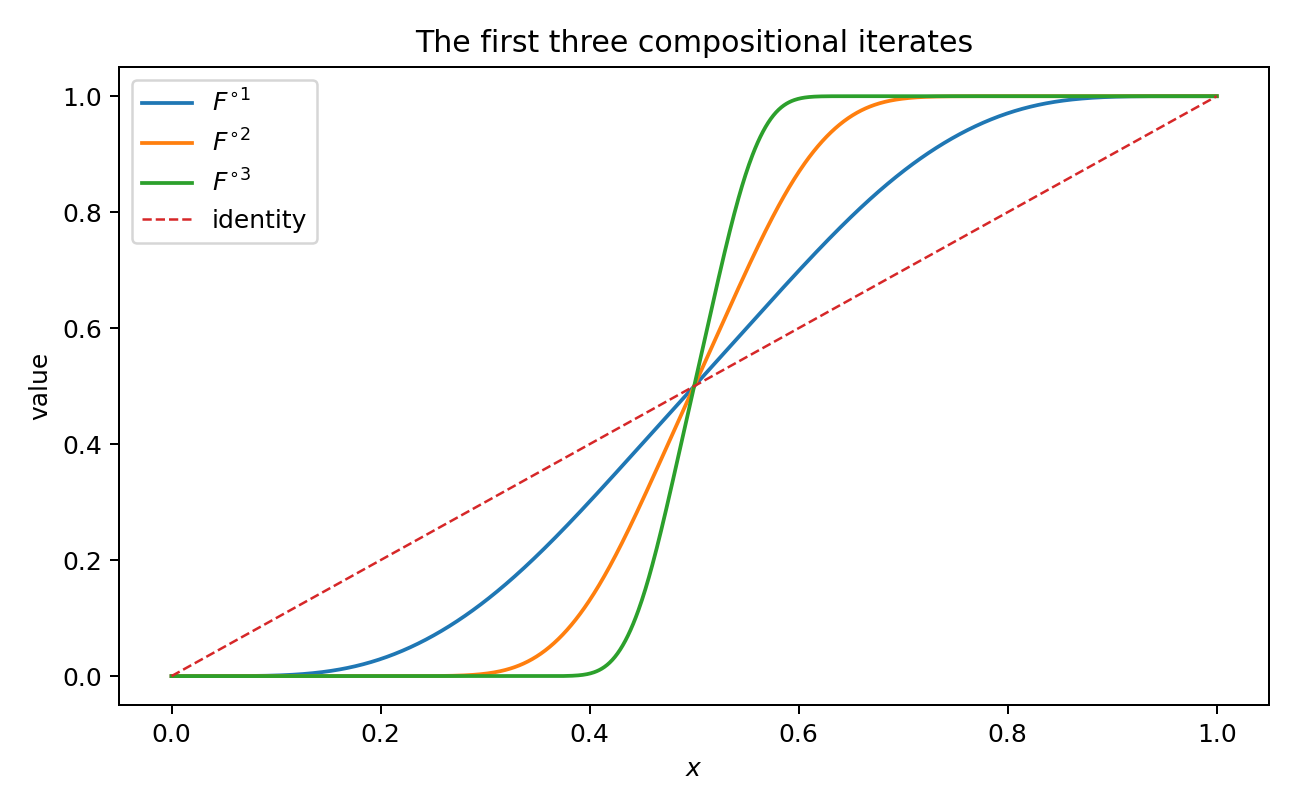
\includegraphics[width=0.86\textwidth]{figures/fabius_iterates.png}
 \caption{Numerical reconstructions of the first three forward compositional iterates.
 The strict drift away from the repelling fixed point $1/2$ and toward the endpoints is
 visible.  The inverse iterates reverse these curves across the diagonal.}
 \label{fig:iterates}
\end{figure}

\subsection{Forward spines and inverse formal reversion}

The default diagnostic uses
\[
 x_0=0.437123456789,\qquad n=4,
 \qquad y_0=G_4(x_0)\approx1.6039811710\times10^{-4}.
\]
The computed orbit and prefix weights are
\begin{align*}
 (x_0,x_1,x_2,x_3)
 &\approx(0.4371234568,0.3743185303,0.2522048636,0.07166875375),\\
 (B_0,B_1,B_2,B_3)
 &\approx(1,1.992844087,3.703442407,3.768767090).
\end{align*}
Thus $j=3$ is the unique dominant forward spine.  Let $D_m$ be the fully composed
forward derivative and $S_m$ the spine sum.  The last two columns below are the
$m$-th roots of the absolute forward and inverse Taylor coefficients.

\begin{table}[htbp]
\centering
\small
\begin{tabular}{@{}rrrrr@{}}
\toprule
$m$ & $D_m/(Q_mH_4^m)$ & $S_m/(Q_mH_4^m)$
& $|[z^m]G_4|^{1/m}$ & $|[w^m]K_4|^{1/m}$\\
\midrule
10 & $ 1.049415$ & $ 0.721343$ & $ 37.84$ & $2.706\times10^3$\\
12 & $-0.503489$ & $-0.378637$ & $ 60.91$ & $3.059\times10^3$\\
13 & $ 0.961480$ & $ 0.998158$ & $ 84.86$ & $3.209\times10^3$\\
15 & $-0.384836$ & $-0.384202$ & $140.94$ & $3.572\times10^3$\\
16 & $-1.008935$ & $-1.002630$ & $200.75$ & $4.727\times10^3$\\
18 & $ 0.432079$ & $ 0.432434$ & $344.83$ & $7.989\times10^3$\\
19 & $-0.998626$ & $-0.999888$ & $486.69$ & $1.118\times10^4$\\
21 & $ 0.091358$ & $ 0.091354$ & $793.50$ & $1.795\times10^4$\\
22 & $ 0.581063$ & $ 0.581018$ & $1176.18$ & $2.644\times10^4$\\
\bottomrule
\end{tabular}
\caption{Finite-order diagnostics.  Oscillation is expected.  The forward theorem
concerns the normalized asymptotic remainder, while the inverse column only illustrates
formal reversion at finite order.}
\label{tab:numerics}
\end{table}

\begin{figure}[htbp]
 \centering
 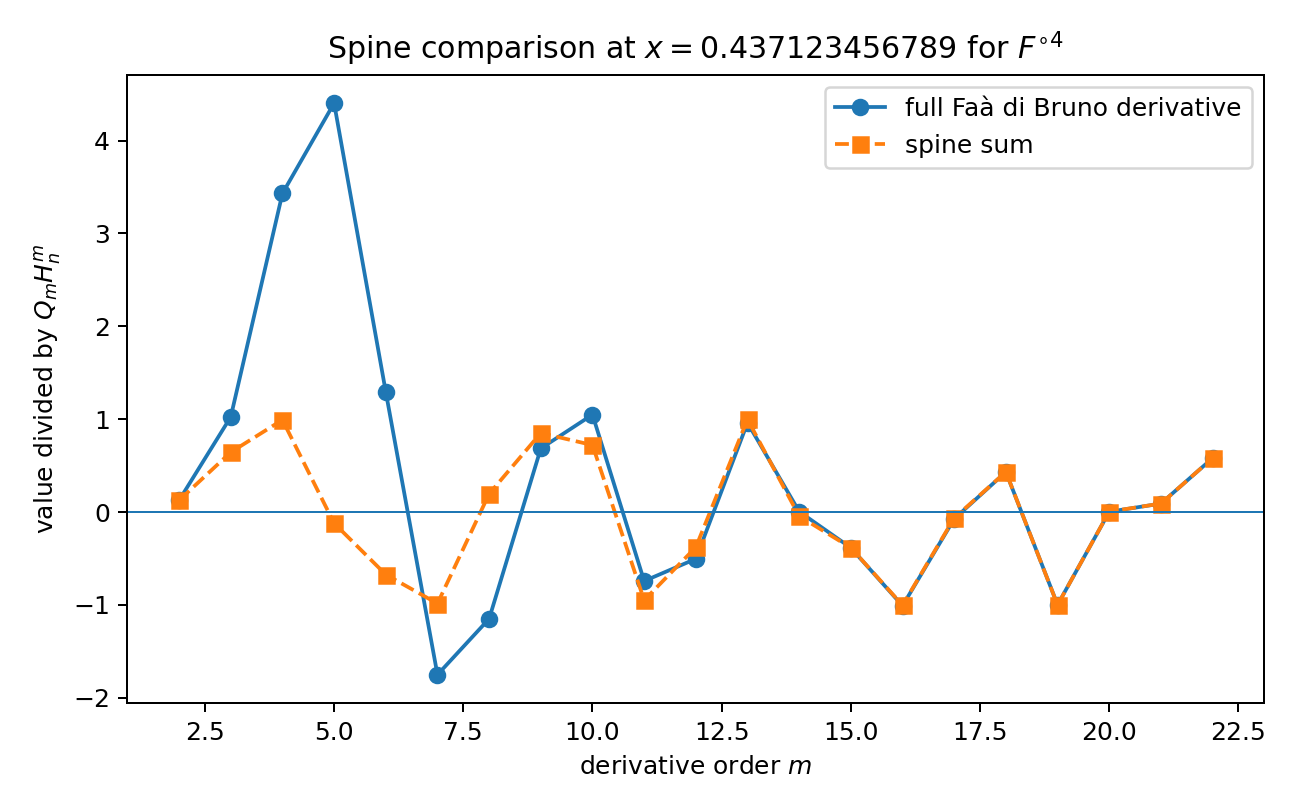
\includegraphics[width=0.86\textwidth]{figures/spine_comparison.png}
 \caption{The full forward derivative and the finite spine sum after normalization by
 $Q_mH_n^m$.}
 \label{fig:spine-comparison}
\end{figure}

\begin{figure}[htbp]
 \centering
 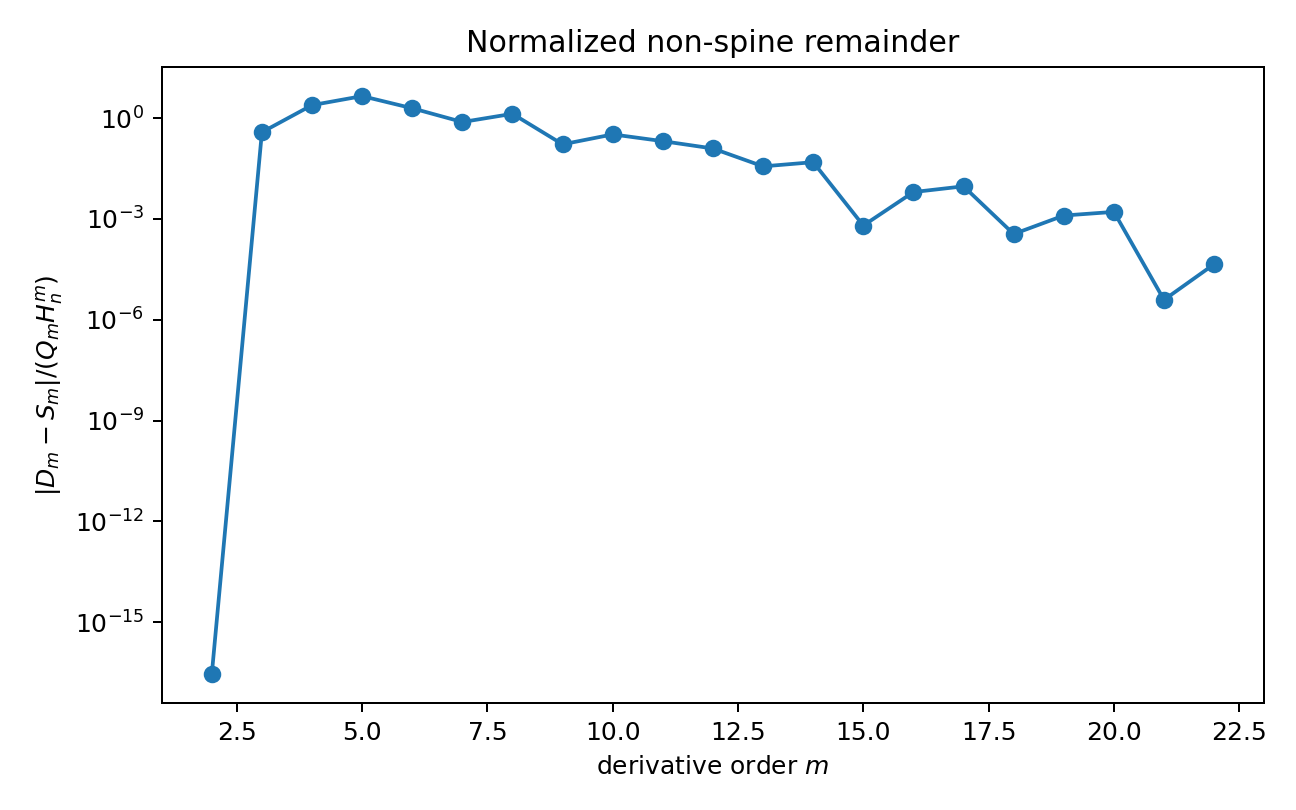
\includegraphics[width=0.86\textwidth]{figures/spine_remainder.png}
 \caption{The normalized non-spine remainder.  The high-order values illustrate the
 defect-driven suppression proved in \cref{prop:defect-decay}.}
 \label{fig:spine-remainder}
\end{figure}

\begin{figure}[htbp]
 \centering
 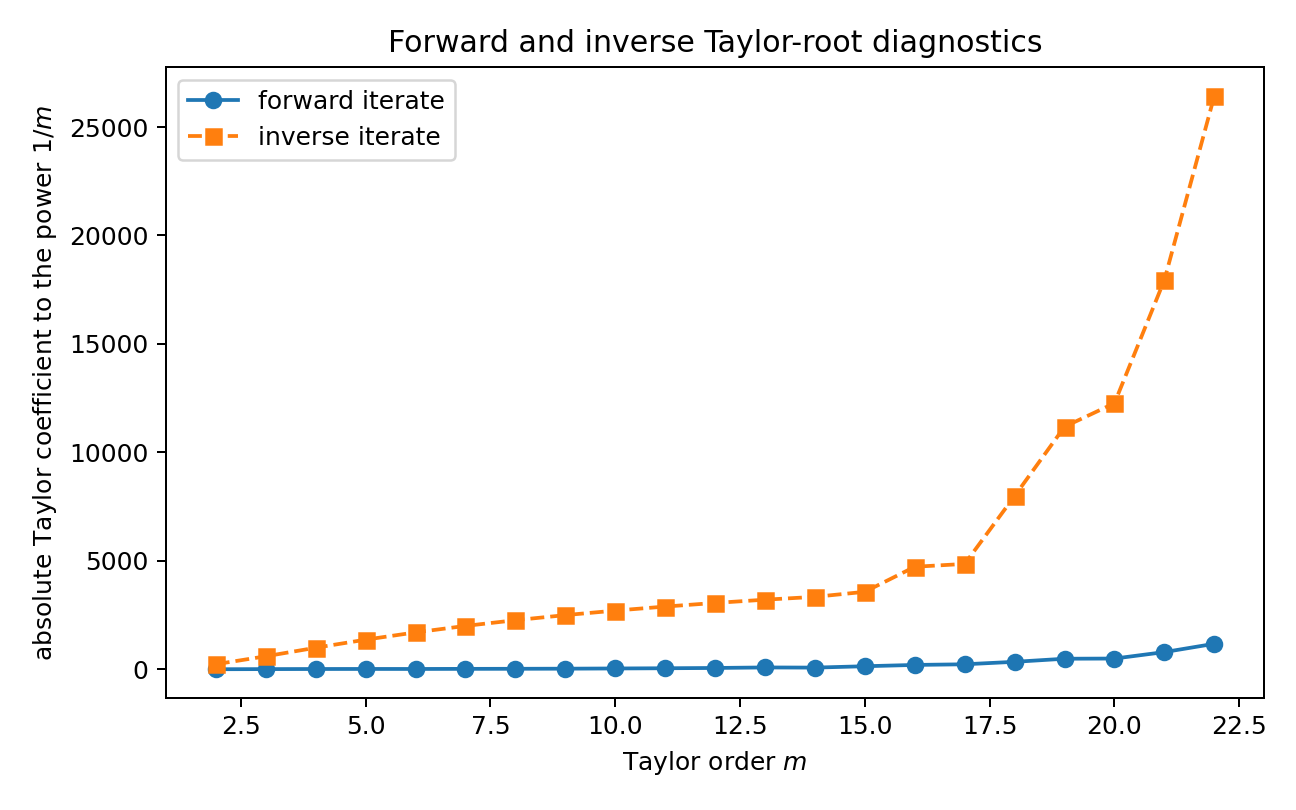
\includegraphics[width=0.86\textwidth]{figures/taylor_root_diagnostic.png}
 \caption{Forward and inverse Taylor-coefficient roots at the paired points
 $x_0$ and $y_0=G_4(x_0)$.  The inverse coefficients are obtained by
 arbitrary-precision formal reversion.}
 \label{fig:taylor-roots}
\end{figure}

\begin{figure}[htbp]
 \centering
 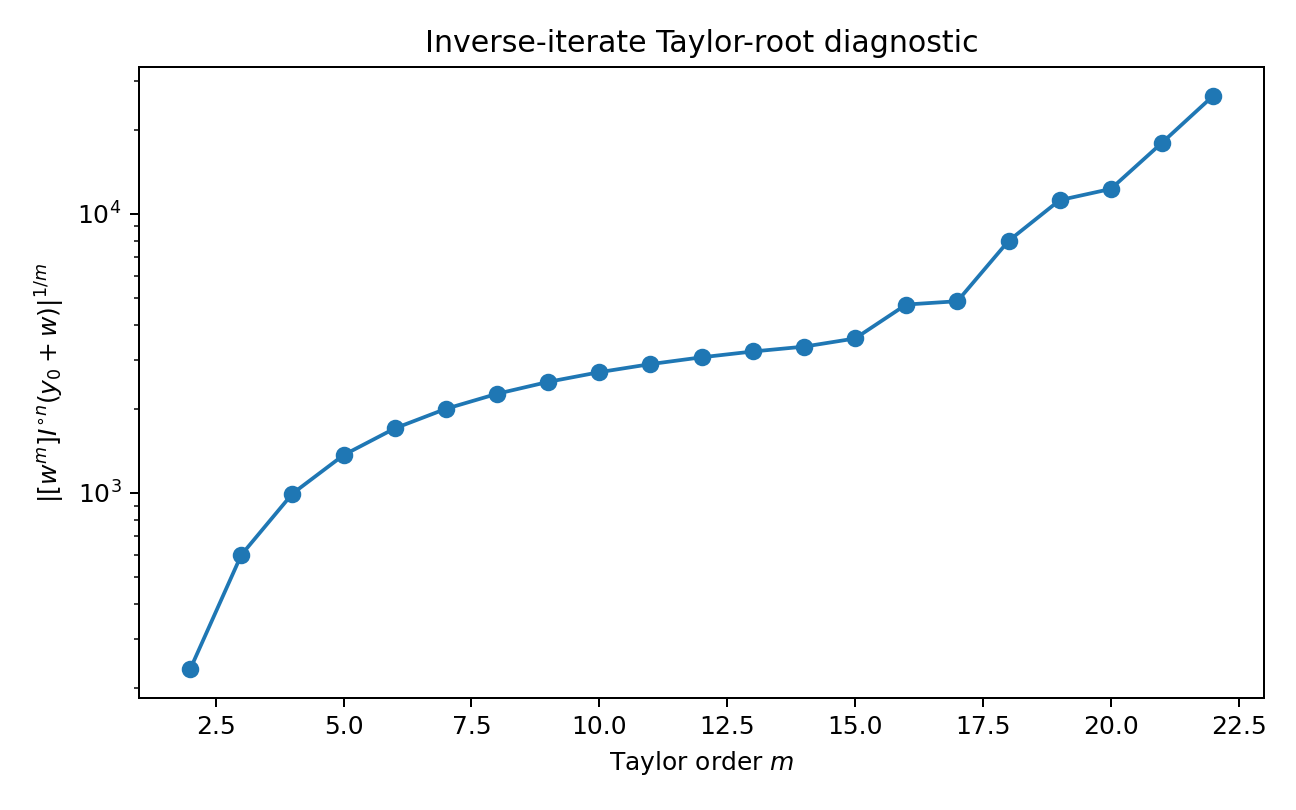
\includegraphics[width=0.86\textwidth]{figures/inverse_taylor_root_diagnostic.png}
 \caption{The inverse-iterate Taylor-root diagnostic alone.  The values are not used to
 infer an asymptotic; they audit the coefficient-reversion implementation and illustrate
 the zero-radius phenomenon proved abstractly.}
 \label{fig:inverse-taylor-roots}
\end{figure}

The script writes all raw values to
\path{numerical_output/spine_diagnostic.csv}, records orbit metadata and the maximum
formal reversion residual, and regenerates every figure.  At degree $22$, using
160 decimal digits, the maximum coefficient residual in
$\widehat G_4\comp\widehat K_4=\id$ is below $2\times10^{-65}$.

\section{Connections to the broader Fabius corpus}
\label{sec:connections}

\subsection{Bell polynomials and Bernoulli cumulants}

Bell polynomials already occur in the repository through moment and cumulant formulae
for dyadic values.  Here the same combinatorial species---set partitions---appears in
a different role: it organizes the derivatives of a composition.  The defect
$D(\pi)$ adds a quadratic dyadic energy to a Bell partition.  This suggests studying
the weighted partition polynomial
\begin{equation}
 \mathcal P_m(z,w)
 :=\sum_{\pi\in\Pi_m}z^{s(\pi)}w^{D(\pi)}.
 \label{eq:defect-polynomial}
\end{equation}
At $w=1$ this collapses toward familiar Bell refinements; at $w=1/2$ it is the exact
suppression factor governing the present proof.  The Bernoulli-cumulant formulas for
$\RvachevUp$ arise from logarithms of dyadic products, while \eqref{eq:defect-polynomial}
measures the combinatorics of composing the resulting quadratic-scale jets.  A
$q$-Bell theory with $q=1/2$ may unify these two appearances.

\subsection{q-binomial and Thue--Morse structure}

The exact dyadic values of $F$ are governed by Gaussian-binomial and q-Pochhammer
identities, whereas the derivative signs in \eqref{eq:dyadic-jet} are Thue--Morse.
The present proof shows that under finite self-composition these structures do not
spread across all Fa\`a di Bruno trees at leading order.  They remain concentrated on
a finite set of orbit spines.  The leading sign-amplitude process is
\begin{equation}
 m\longmapsto
 \ThetaF(2^m x_{j_*}),
 \label{eq:leading-symbolic-process}
\end{equation}
which is a direct symbolic sampling of the dyadic shift.  Thus a high-dimensional
Bell expansion asymptotically collapses to a one-dimensional Thue--Morse-modulated
orbit observable.

\subsection{Infinite sinc products}

The sinc product \eqref{eq:sinc-product} supplies the numerical representation used
here and explains the exceptional smoothness of $\RvachevUp$.  The nowhere-analyticity
mechanism, however, is most transparent in physical space: dilation creates $Q_m$,
block translation creates Thue--Morse signs, and binary transitions prevent the
amplitude from becoming too small forever.  The Fourier and derivative pictures are
therefore complementary.  A possible future goal is to derive the spine expansion
directly from a multidimensional Fourier integral for $F^{\comp n}$, but nonlinear
composition makes such a representation substantially less direct than the
set-partition proof.

\subsection[Lambert-W endpoint asymptotics]{Lambert--$W$ endpoint asymptotics}

The repository develops the small-argument asymptotic of $F$ in a phase variable
encoded by the lower real branch $W_{-1}$.  Inverting once turns the quadratic
logarithmic scale into a square-root logarithmic scale; iterating $n$ times repeatedly
halves the logarithmic exponent, as proved in \cref{thm:iterated-endpoint}.
The full expansion is subtler: its bounded period-one phase survives inversion and
should be evaluated at a nested sequence of Lambert phases.  This produces a natural
hierarchy
\[
 T\mapsto\sqrt{2(\log2)T}\mapsto
 \sqrt{2(\log2)\sqrt{2(\log2)T}}\mapsto\cdots,
\]
with lower-order logarithms and periodic corrections at every level.  A uniform
all-orders theorem for this nested hierarchy would refine the endpoint part of the
present report and could quantify the blow-up of $K_n'$ and its higher derivatives.

\subsection{Legendre expansions and polynomial representations}

The Rvachev function admits rapidly convergent orthogonal-polynomial expansions, and
the repository develops finite representations of polynomials by shifted copies of
$\RvachevUp$.  Forward iterates become increasingly step-like about $1/2$ as $n$ grows, while
inverse iterates become increasingly flat in the center and increasingly steep near the
endpoints.  Their Legendre coefficients should therefore have complementary two-scale
regimes.  Nowhere analyticity rules out geometric coefficient decay strong enough to
produce a Bernstein-ellipse extension across any real subinterval.  The endpoint law
\eqref{eq:iterated-inverse-endpoint} suggests that the inverse coefficients may be
controlled by stretched-logarithmic saddle points rather than an ordinary algebraic or
exponential scale.  Determining that scale would connect local inverse singularity to
global polynomial approximation.

\section{Conjectures and research directions}
\label{sec:future}

The main theorem is complete, but it leaves a structured exceptional countable set on
which the formal Taylor series may converge without representing the function.  The
formal-radius transport theorem shows that the inverse classification is exactly the
homeomorphic image of the forward positive-radius locus.  Of the five submitted
conjecture environments, only two remain live manuscript conjectures.  Three are
retained as explicit warning records: one has a false inverse clause, one is already
proved from exact quarter-point facts, and one duplicates the corrected forward
report's sole live conjecture.  Neither live conjecture has an exact proved Lean
counterpart.

\begin{warning}[Former Conjecture 14.1 has a false inverse clause]
\label{warn:trichotomy}
The submitted statement first proposed that the positive-radius locus of $G_n$ is
precisely its eventually-zero-jet locus, then claimed that
\cref{thm:formal-reversion} gives the same eventual-zero classification for $K_n$.
The second clause is false: formal reversion preserves convergence, not polynomiality.
At $x=1/4$ the exact forward Taylor germ is
\[
 \widehat F_{1/4}(z)=\frac5{72}+z+4z^2,
\]
because $F'(1/4)=1$, $F''(1/4)=8$, and all higher derivatives vanish.  At
$y=F(1/4)=5/72$, the inverse Taylor germ therefore solves $w=z+4z^2$ and is
\[
 z=\frac{\sqrt{1+16w}-1}{8},
\]
an infinite convergent series.  Thus $K_1=I$ has positive Taylor radius at $5/72$
without an eventually-zero jet.  The forward-only assertion remains a plausible open
classification problem, especially for $n\geq2$, but no inverse eventual-zero
equivalence is asserted here.
\end{warning}

The center is exceptional in both directions because its forward and inverse formal
series are affine.  At noncentral dyadic points for $n=1$, however, finite nonlinear
forward Taylor polynomials revert to infinite convergent inverse series, exactly as the
quarter-point example shows.

\begin{warning}[Former Conjecture 14.2 is already discharged]
\label{warn:ties}
The submitted tie-cancellation statement is not a live conjecture.  If
$x\in T_n$, the tied adjacent weights satisfy $a_k=1$.  Strict monotonicity of $F'$,
together with $F'(1/4)=F'(3/4)=1$, forces
$x_k\in\{1/4,3/4\}$.  Hence
$x_{k+1}=F(x_k)\in\{5/72,67/72\}$.  The first orbit point is dyadic, so
$\ThetaF(2^m x_k)=0$ for every sufficiently large $m$ by
\eqref{eq:dyadic-jet}; the second is non-dyadic, so
\cref{lem:binary-transition} supplies infinitely many $m$ with
$\AbsoluteValue{\ThetaF(2^m x_{k+1})}\geq1/2$.  Since the fixed suffix coefficient
$A_{k+1,n}$ is positive, along that subsequence the surviving tied spine term has
absolute value at least $(A_{k+1,n}/2)H_n(x)^m$.  Thus persistent cancellation is
already excluded by exact quarter-point facts and the binary-transition lemma; no
additional Thue--Morse correlation conjecture remains.
\end{warning}

\begin{conjecture}[Direct inverse-spine asymptotic]
\label{conj:inverse-spine}
For $y=G_n(x)$ away from an explicit countable exceptional set, the derivatives of
$K_n$ admit an asymptotic expansion on the same universal quadratic scale $Q_m$,
\[
 K_n^{(m)}(y)=Q_m\left[
   \sum_{j=0}^{n-1}\widetilde A_{j,n}(x)
   \widetilde B_j(x)^m\Theta(2^m x_j)
   +o(\widetilde H_n(x)^m)
 \right],
\]
with computable inverse prefix weights $\widetilde B_j$ obtained from the forward
slopes and with a unique dominant term off finite tie surfaces.
\end{conjecture}

The implicit identity $G_n\comp K_n=\id$ and the same partition defect provide a
plausible route, but one must control the recursive inverse Bell polynomials without
assuming the desired envelope.  A proof would upgrade abstract zero-radius transport
to explicit derivative lower bounds for the inverse iterates.  The finite-order replay
does not establish the displayed scale, weights, exceptional set, or remainder.

\begin{warning}[Former Conjecture 14.4 duplicates the forward report]
\label{warn:defect-duplicate}
The submitted statement that, for every fixed $z>0$, the weighted partition sums
\[
 \sum_{\substack{\pi\in\Pi_m\\1<|\pi|<m}}z^{s(\pi)}2^{-D(\pi)}
\]
admit a full asymptotic expansion whose leading term comes from the two first-defect
shells: one block of size $2$ with the rest singleton, and one block of size $m-1$ with
one singleton is exactly Conjecture 14.3 of the corrected forward-iterate report.
It remains open manuscript mathematics there, with no exact Lean counterpart, but it
is not a second independent inverse-iterate conjecture.  A sharp version would give an
explicit two-spine rate and the first correction term for both forward and prospective
inverse spines.
\end{warning}

\begin{conjecture}[Nested Lambert phase law]
\label{conj:nested-lambert}
The repository's all-orders endpoint expansion for $I$ can be iterated a fixed number
of times to produce an all-orders transseries for $K_n$ whose coefficient functions are
smooth and periodic in a hierarchy of nested lower-branch Lambert phases.  The leading
term is \eqref{eq:iterated-inverse-endpoint}, and each iteration transports rather than
erases the dyadic periodic ripple.
\end{conjecture}

This all-orders claim is not implied by the proved leading scale, has not been tested by
the interior Taylor-reversion experiment, and has no exact Lean counterpart.

\subsection{Promising formalization route}

A Lean formalization can be modular.
\begin{enumerate}[label=\arabic*.]
 \item Define $Q_m$ and formalize the partition defect and the exact factorization
 \eqref{eq:Q-factorization}.
 \item Prove a sufficiently explicit weighted defect bound for finite set partitions.
 \item Use the existing derivative atlas and bounded-derivative API to formalize the
 two-spine reduction and the fixed-$n$ orbit-spine induction.
 \item Reuse strict monotonicity, convexity, and order-isomorphism modules to prove the
 finite tie-set and dense dominant-amplitude statements.
 \item Finish the forward theorem with the existing power-series radius and analytic-at
 infrastructure.
 \item Formalize the purely algebraic uniqueness of the compositional inverse of a
 formal power series with invertible linear coefficient.
 \item Combine the analytic inverse-function theorem with formal-series convergence to
 prove \cref{thm:formal-reversion} and transport $E_n$ to $Y_n$.
 \item Import the formal quadratic endpoint law and prove the elementary induction for
 \cref{thm:iterated-endpoint}.
\end{enumerate}
The formal-reversion layer should be reusable well beyond the Fabius development.

\subsection{Generalization to other atomic functions}

The proof abstracts beyond the classical dyadic case.  Suppose a smooth increasing map
$f$ has derivatives
\begin{equation}
 f^{(m)}(x)=q^{\binom{m+1}{2}}\Phi(q^m x),
 \label{eq:q-atomic-derivatives}
\end{equation}
for some $q>1$, with bounded $\Phi$, recurrent nonvanishing along a dense set of
$q$-adic orbits, and monotone orbit slopes yielding a unique dominant prefix.  The same
partition calculation replaces $2^{-D(\pi)}$ by $q^{-D(\pi)}$.  Once forward iterates
are controlled, \cref{thm:formal-reversion} automatically transfers every zero-radius
statement to inverse iterates.  This suggests a general theorem for invertible
Rvachev-type distribution functions and multiscale refinable maps.

\section{Summary of the proof mechanism}

The complete argument can be compressed into the following chain.
\begin{enumerate}[label=\arabic*.]
 \item Exact differentiation gives
 $F^{(m)}=Q_m\Theta\comp(2^m\cdot)$ with
 $Q_m=2^{m(m+1)/2}$ and $|\Theta|\leq1$.
 \item In Fa\`a di Bruno's set-partition formula, every non-spine partition has a
 positive quadratic defect $D(\pi)$.
 \item The weighted sum of all non-spine partitions is exponentially small despite
 Bell-number multiplicity.
 \item Hence, after division by $Q_m$, the derivative $G_n^{(m)}$ is asymptotic to a
 finite sum of orbit spines:
 \
 \[
   A_{j,n}B_j^m\Theta(2^m x_j),\qquad 0\leq j<n.
 \]
 \item Away from a finite tie set, monotone orbit dynamics makes one $B_j$ uniquely
 maximal; away from countably many dyadic orbit preimages, binary transitions keep its
 amplitude at least $1/2$ infinitely often.
 \item Therefore $R_{G_n}(x)=0$ on a co-countable dense set $E_n$, and $G_n$ is nowhere
 analytic.
 \item Smooth local inverse Taylor series are unique formal compositional inverses.
 Positive convergence radius is invariant under reversion.
 \item Thus $R_{K_n}(y)=0$ on the co-countable dense set $Y_n=G_n(E_n)$, and no interior
 point of $K_n$ can be analytic.
 \item At the endpoints, $K_n(y)/y^\alpha\to\infty$ for every $\alpha>0$; hence endpoint
 analyticity is impossible.  At the center, the Taylor series is affine but does not
 represent the function.
\end{enumerate}
This proves \cref{thm:inverse-main,thm:inverse-strong} and explains why finite
self-composition cannot regularize either the Fabius function or its inverse.

\appendix

\section{Auxiliary details on the partition defect}
\label{app:defect}

This appendix records two identities useful for sharpening
\cref{prop:defect-decay}.

\begin{proposition}[Exact minimum at fixed block count]
\label{prop:fixed-k-minimum}
Among partitions of $m$ with $k$ blocks,
\begin{equation}
 \min D(\pi)=(k-1)(m-k).
 \label{eq:fixed-k-minimum}
\end{equation}
Equality holds exactly when one block has size $m-k+1$ and every other block is a
singleton.
\end{proposition}

\begin{proof}
For fixed $m,k$, formula \eqref{eq:defect} shows that minimizing $D$ is equivalent to
maximizing $\sum_i\binom{r_i}{2}$.  Strict convexity of $r\mapsto\binom r2$ transfers
one unit from a smaller nonsingleton block to a larger block and increases the sum.
Iteration leaves one large block and $k-1$ singletons.  Direct substitution gives
\eqref{eq:fixed-k-minimum}.
\end{proof}

\begin{proposition}[First defect shell]
\label{prop:first-shell}
For $m\geq3$, the least positive defect is $m-2$.  It occurs for exactly two block-size
profiles:
\begin{equation}
 (2,1,\ldots,1)
 \qquad\text{and}\qquad
 (m-1,1).
 \label{eq:first-shell}
\end{equation}
\end{proposition}

\begin{proof}
From \eqref{eq:fixed-k-minimum}, the least positive value over $2\leq k\leq m-1$ is
\[
 \min_{2\leq k\leq m-1}(k-1)(m-k)=m-2,
\]
attained only at $k=2$ and $k=m-1$.  The equality classification in
\cref{prop:fixed-k-minimum} gives the two profiles.
\end{proof}

This identifies the candidate leading correction to the spine sum.  At the
near-singleton end, choose one pair and leave all other elements singleton; at the
near-giant end, choose the singleton outside a block of size $m-1$.  Both carry the
same dyadic penalty $2^{-(m-2)}$, but their derivative coefficients and orbit factors
are different.  A refined expansion should sum these shells before estimating the
higher-defect remainder.

\section{Reproducibility guide}
\label{app:reproducibility}

The archive contains the following files.
\begin{longtable}{@{}>{\raggedright\arraybackslash}p{0.40\textwidth}>{\raggedright\arraybackslash}p{0.52\textwidth}@{}}
\toprule
File & Purpose\\
\midrule
\endhead
\texttt{inverse\_fabius\_iterates\_}\newline\texttt{nowhere\_analytic.tex}
& Complete LaTeX source of this report.\\
\texttt{inverse\_fabius\_iterates\_}\newline\texttt{nowhere\_analytic.pdf}
& Rendered report.\\
\path{numerical_experiments.py}
& Commented Python program for sinc-product reconstruction, forward Taylor
composition, arbitrary-precision inverse-series reversion, spine evaluation, CSV
output, and figures.\\
\texttt{numerical\_output/}\newline\texttt{spine\_diagnostic.csv}
& Raw forward derivative, spine, inverse coefficient, and formal-reversion
residual diagnostics through the selected maximum order.\\
\texttt{numerical\_output/}\newline\texttt{numerical\_metadata.txt}
& Parameters, paired points, orbit points, slopes, prefixes, suffixes, dominant
weight, and maximum formal-reversion residual.\\
\path{figures/*.png}
& Figures included in the report.\\
\bottomrule
\end{longtable}

A typical reproduction command is
\begin{lstlisting}[style=pseudo,language=bash]
python numerical_experiments.py \
  --output-dir numerical_output \
  --x0 0.437123456789 \
  --iterate-count 4 \
  --max-order 22
\end{lstlisting}
The program requires Python 3, NumPy, SciPy, Matplotlib, and mpmath.  It performs consistency
checks at $\RvachevUp(0)$, $\RvachevUp(1/2)$, $F(0)$, $F(1/2)$, and $F(1)$ before writing output.

\section{Repository source map}
\label{app:source-map}

Under the common root \path{Analysis/FabiusFunction/}, the repository paths most
directly connected to the proof are:
\begin{itemize}[leftmargin=2em]
 \item \path{docs/Fabius_Function_and_Rvachev_Up/}
 for the primary exposition;
 \item \path{GlobalExtension.lean}
 and \path{BoundedDerivatives.lean} in \path{Lean/FabiusFunction/} for the derivative atlas;
 \item \path{Convexity.lean}, \path{Monotonicity.lean}, and the order-isomorphism
 modules for the orbit dynamics;
 \item \path{OriginalPaperSupplement.lean} and \path{NowhereAnalytic.lean} for the
 base nonanalyticity proof;
 \item \path{docs/Non_Elementarity_of_the_Fabius_Function/} for the exact
 analytic-locus obstruction for both $F$ and $I$;
 \item \path{docs/semi-formalized-research-frontiers/} for q-series, Bell/Bernoulli,
 sinc-product, Lambert--$W$, Legendre, and other frontier connections;
 \item \path{docs/archive/} and the frontier README for provenance and consolidation
 of historical TeX drafts.
\end{itemize}

\footnotesize
\begin{thebibliography}{99}

\bibitem{Fabius1966}
J.~Fabius,
\newblock A probabilistic example of a nowhere analytic $C^\infty$-function,
\newblock \emph{Z. Wahrscheinlichkeitstheorie verw. Geb.} \textbf{5} (1966),
173--174.

\bibitem{Arias1982}
J.~Arias de Reyna,
\newblock An infinitely differentiable function with compact support: definition and
properties,
\newblock English translation of \emph{Rev. Real Acad. Ciencias Madrid} \textbf{76}
(1982), 21--38, arXiv:1702.05442.

\bibitem{AriasArithmetic}
J.~Arias de Reyna,
\newblock Arithmetic of the Fabius function,
\newblock arXiv:1702.06487v3, 2017.

\bibitem{Comtet}
L.~Comtet,
\newblock \emph{Advanced Combinatorics: The Art of Finite and Infinite Expansions},
\newblock revised and enlarged edition, D. Reidel, 1974.

\bibitem{Johnson2002}
W.~P. Johnson,
\newblock The curious history of Fa\`a di Bruno's formula,
\newblock \emph{American Mathematical Monthly} \textbf{109} (2002), 217--234.

\bibitem{KrantzParks}
S.~G. Krantz and H.~R. Parks,
\newblock \emph{A Primer of Real Analytic Functions},
\newblock second edition, Birkh\"auser, 2002.

\bibitem{Henrici}
P.~Henrici,
\newblock \emph{Applied and Computational Complex Analysis, Vol.~1},
\newblock Wiley, 1974; see the chapters on power-series reversion and the analytic
inverse-function theorem.

\bibitem{ProveItPrimary}
V.~Reshetnikov,
\newblock \emph{The Fabius Function and Rvachev's Up Function},
\newblock proof-backed primary exposition in the ProveIt repository,
\newblock \url{https://github.com/VladimirReshetnikov/ProveIt/tree/main/Analysis/FabiusFunction},
accessed 30 August 2026.


\end{thebibliography}

\end{document}
